\chapter{Results}
\label{chapter:results}

Quantitative evaluations were performed on the results, and qualitative evaluations were performed on some graphs, including visualizations of embeddings, for all experiments defined in the Experimental Setup (see Chapter \ref{chapter:exp_setup}), including \ac{SL} and \ac{DL} models, with and without pre-training, in different label scarcity modalities and showing ORDER anomaly detection. Approximately 100 experiments were performed for each dataset. Therefore, only the experiment with the best metric, according to F1 Weighted without anomalies, for each dataset was shown in more detail. The experiments were conducted on the three datasets created: Brazil, California, and Texas. 

\section{Shallow and Deep Baselines for SITS}

Initially, a baseline was established by training all \ac{SL} and \ac{DL} models in a fully supervised manner, using 70\% of the data for training. Tables \ref{tab:res_scratch_brazil}, \ref{tab:res_scratch_california}, and \ref{tab:res_scratch_texas} present the Weighted F1, Accuracy, Specificity, G-Mean, ConfidNet metrics in the \ac{DL} and \ac{MLP} models (including False Positive Rates, AUC and AUPR), for the Brazil, California, and Texas datasets, respectively. This discrepancy highlights the superior capability of deep architectures, particularly Transformers and State Space Models (Mamba), in capturing complex temporal dependencies in spectrally similar classes, which are abundant in the tropical agriculture of Brazil. Also, compairing Max Class Probability AUC with ConfidNet AUC, it is well known that the results vary; sometimes the model itself is better, sometimes ConfidNet is better. This shows that ConfidNet presented poor results, since the strategy is specifically designed to generate a better Precision-Recall curve than the original model.

\begin{table}[ht!]
\centering
\caption{Training results from scratch using 70\% on training data in the Brazil dataset.}
\label{tab:res_scratch_brazil}
\resizebox{\textwidth}{!}{%
\begin{tabular}{lccccccccccccc}
\hline
\textbf{Model} & \textbf{} & \textbf{} & \textbf{} & \textbf{} & \textbf{G} & \textbf{Mcp} & \textbf{} & \textbf{Conf} & \textbf{AUPR} & \textbf{AUPR} & \textbf{Conf} & \textbf{Anom} & \textbf{w. A} \\
 & \textbf{F1} & \textbf{Acc} & \textbf{Spec} & \textbf{Mcc} & \textbf{Mea} & \textbf{Auc} & \textbf{Fpr95} & \textbf{Auc} & \textbf{S} & \textbf{E} & \textbf{AUPR} & \textbf{Rate} & \textbf{F1} \\ \hline
SVM & 77.7 & 78.3 & 97.4 & 74.3 & 89.9 & - & - & - & - & - & - & \textbf{2.6} & 78.5 \\
RF & 75.0 & 76.0 & 97.0 & 71.6 & 86.3 & - & - & - & - & - & - & \textbf{1.3} & 75.0 \\
LGBM & 78.0 & 78.8 & 97.4 & 74.7 & 89.5 & - & - & - & - & - & - & 4.3 & 77.9 \\
MLP & 79.2 & 80.0 & 97.6 & 76.4 & 90.6 & 80.5 & 64.0 & 76.3 & 92.6 & 41.1 & \textbf{65.0} & 6.6 & 80.2 \\ \hline
CNN & 83.8 & 84.0 & 98.1 & 80.9 & 91.7 & 81.8 & 63.6 & 82.8 & 95.7 & 46.1 & \textbf{61.5} & 4.2 & 85.3 \\
LSTM & 84.6 & 84.5 & 98.1 & 81.4 & 91.9 & 82.5 & \textbf{60.1} & \textbf{84.6} & \textbf{96.3} & \textbf{49.2} & 56.0 & 5.7 & 85.8 \\
BERT & 84.1 & 84.0 & 98.1 & 80.9 & \textbf{92.3} & 80.9 & 65.3 & 83.1 & 95.8 & 47.0 & 60.3 & 5.6 & 85.8 \\
BERT++ & \textbf{85.6} & \textbf{85.5} & \textbf{98.3} & \textbf{82.7} & \textbf{92.7} & \textbf{82.9} & 60.8 & \textbf{84.0} & \textbf{96.2} & \textbf{48.1} & 60.1 & 6.3 & \textbf{87.3} \\
MAMBA & \textbf{85.0} & \textbf{85.1} & \textbf{98.2} & \textbf{82.2} & 92.2 & \textbf{83.2} & \textbf{59.7} & 82.9 & \textbf{96.2} & 44.2 & 55.8 & 3.4 & \textbf{85.9} \\ \hline
\end{tabular}%
}
\end{table}

\begin{table}[ht!]
\centering
\caption{Training results from scratch using 70\% on training data in the Texas dataset.}
\label{tab:res_scratch_texas}
\resizebox{\textwidth}{!}{%
\begin{tabular}{lccccccccccccc}
\hline
\textbf{Model} & \textbf{} & \textbf{} & \textbf{} & \textbf{} & \textbf{G} & \textbf{Mcp} & \textbf{} & \textbf{Conf} & \textbf{AUPR} & \textbf{AUPR} & \textbf{Conf} & \textbf{Anom} & \textbf{w. A} \\
 & \textbf{F1} & \textbf{Acc} & \textbf{Spec} & \textbf{Mcc} & \textbf{Mea} & \textbf{Auc} & \textbf{Fpr95} & \textbf{Auc} & \textbf{S} & \textbf{E} & \textbf{AUPR} & \textbf{Rate} & \textbf{F1} \\ \hline
SVM & 98.8 & 98.8 & \textbf{99.8} & 98.4 & 98.9 & - & - & - & - & - & - & \textbf{0.1} & 98.9 \\
RF & 97.9 & 98.0 & 99.6 & 97.3 & 96.2 & - & - & - & - & - & - & \textbf{0.1} & 97.9 \\
LGBM & 98.9 & 98.9 & \textbf{99.8} & 98.5 & 98.2 & - & - & - & - & - & - & \textbf{0.1} & 98.9 \\
MLP & 99.1 & 99.1 & \textbf{99.8} & 98.8 & 99.2 & 96.2 & 20.4 & \textbf{76.2} & \textbf{99.6} & \textbf{3.1} & 80.9 & \textbf{0.2} & 99.2 \\ \hline
CNN & \textbf{99.5} & \textbf{99.5} & \textbf{99.9} & \textbf{99.4} & 99.4 & \textbf{97.7} & \textbf{7.8} & 51.7 & 99.5 & 0.5 & 98.3 & \textbf{0.1} & \textbf{99.6} \\
LSTM & \textbf{99.6} & \textbf{99.6} & \textbf{99.9} & \textbf{99.5} & \textbf{99.5} & \textbf{97.7} & \textbf{7.8} & 35.5 & 99.4 & 0.3 & \textbf{99.0} & \textbf{0.1} & \textbf{99.7} \\
BERT & \textbf{99.5} & \textbf{99.5} & \textbf{99.9} & 99.3 & 99.4 & 96.9 & 15.0 & 33.2 & 99.1 & 0.4 & \textbf{99.3} & \textbf{0.1} & 99.5 \\
BERT++ & \textbf{99.5} & \textbf{99.5} & \textbf{99.9} & \textbf{99.4} & \textbf{99.5} & 96.9 & 13.6 & \textbf{89.4} & \textbf{99.9} & \textbf{21.2} & 52.7 & \textbf{0.2} & \textbf{99.6} \\
MAMBA & \textbf{99.6} & \textbf{99.6} & \textbf{99.9} & \textbf{99.5} & \textbf{99.6} & \textbf{98.4} & \textbf{6.3} & 45.4 & \textbf{99.6} & 0.3 & 97.4 & \textbf{0.1} & \textbf{99.7} \\ \hline
\end{tabular}%
}
\end{table}

\begin{table}[ht!]
\centering
\caption{Training results from scratch using 70\% on training data in the California dataset.}
\label{tab:res_scratch_california}
\resizebox{\textwidth}{!}{%
\begin{tabular}{lccccccccccccc}
\hline
\textbf{Model} & \textbf{} & \textbf{} & \textbf{} & \textbf{} & \textbf{G} & \textbf{Mcp} & \textbf{} & \textbf{Conf} & \textbf{AUPR} & \textbf{AUPR} & \textbf{Conf} & \textbf{Anom} & \textbf{w. A} \\
 & \textbf{F1} & \textbf{Acc} & \textbf{Spec} & \textbf{Mcc} & \textbf{Mea} & \textbf{Auc} & \textbf{Fpr95} & \textbf{Auc} & \textbf{S} & \textbf{E} & \textbf{AUPR} & \textbf{Rate} & \textbf{F1} \\ \hline
SVM & 97.2 & 97.2 & \textbf{99.8} & 96.7 & 98.2 & - & - & - & - & - & - & 0.9 & 7.4 \\
RF & 95.3 & 95.3 & 99.6 & 94.5 & 96.4 & - & - & - & - & - & - & \textbf{0.3} & 95.3 \\
LGBM & 96.2 & 96.2 & 99.7 & 95.6 & 97.7 & - & - & - & - & - & - & 1.2 & 96.7 \\
MLP & 97.0 & 97.0 & \textbf{99.8} & 96.5 & \textbf{98.6} & 92.9 & 41.8 & 59.3 & 98.2 & 3.4 & \textbf{76.8} & 1.0 & 97.5 \\ \hline
CNN & \textbf{98.2} & \textbf{98.2} & \textbf{99.8} & \textbf{97.9} & \textbf{98.6} & 95.3 & 22.5 & \textbf{94.8} & \textbf{99.9} & 36.4 & 25.9 & 0.7 & \textbf{98.2} \\
LSTM & 97.4 & 97.4 & \textbf{99.8} & 97.0 & 97.2 & \textbf{95.4} & \textbf{19.0} & \textbf{95.6} & \textbf{99.9} & \textbf{49.1} & 19.9 & 1.0 & 97.9 \\
BERT & \textbf{98.0} & \textbf{98.0} & \textbf{99.8} & \textbf{97.6} & 98.5 & \textbf{95.7} & \textbf{16.6} & 32.6 & 96.9 & 1.4 & \textbf{97.8} & \textbf{0.5} & \textbf{98.2} \\
BERT++ & 97.7 & 97.7 & \textbf{99.8} & 97.4 & \textbf{98.6} & 95.1 & 21.3 & 94.1 & \textbf{99.8} & \textbf{42.7} & 27.9 & 1.4 & \textbf{98.1} \\
MAMBA & 97.9 & 97.9 & \textbf{99.8} & \textbf{97.6} & \textbf{98.8} & \textbf{95.4} & 19.7 & 90.9 & 99.7 & 31.3 & 50.1 & 0.8 & 98.0 \\ \hline
\end{tabular}%
}
\end{table}

As expected, it was noted that the Brazilian dataset presents the worst metrics in all models when compared to those from Texas and California. In the Brazil dataset (see \autoref{tab:res_scratch_brazil}), the best \ac{DL} models (SITS-BERT++ and SITS-Mamba) achieved a Weighted F1 score of around 85\%, while the \ac{SL} models (such as SVM and LGBM) scored below 80\%. This increase also occurred, but to a lesser extent, in the California dataset (see \autoref{tab:res_scratch_california}), where \ac{DL} models such as SITS-BERT and SITS-LSTM were close to 98\% F1 Weighted, while \ac{SL} models were close to 95\%, with the exception of \ac{SVM}, which remained partially competitive with around 97\%. The reduced gap between SL and DL in California suggests that the spectral separability of crops in this region is naturally higher, allowing even simpler models like \ac{SVM} to find good decision boundaries. The Texas dataset (see \autoref{tab:res_scratch_texas}) was the easiest, with architectures such as SITS-LSTM and SITS-ConvNeXt achieving metrics above 99\%, with \ac{SVM} also remaining competitive with a Weighted F1 score close to 99\%. 

As for the results referring to the ConfidNet anomaly detection baseline, the opposite occurred: the metrics were worse for the California and Texas datasets, following what was observed by \cite{cheng2019leveraging} that the methodology tends not to work if the model makes classifications with very high result metrics. This happens because, in highly evaluation metric models, the confidence scores for both correct and incorrect predictions tend to cluster near 1 (overconfidence), making it difficult for the threshold-based approach of ConfidNet to distinguish between in-distribution errors and anomalies (as pointed out by the authors of the mod). Our ORDER method, on the other hand, showed solid results, improving the Weighted F1 metrics in all \ac{DL} models and in almost all \ac{SL} models, with the only exceptions being \ac{RF} and \ac{LGBM} in the California dataset (see \autoref{tab:res_scratch_california}).

\section{Pre-training analysis}

Before finetuning the pre-trained models on target data, the quality of the embeddings generated by the SSL strategies (Masked Modeling - MM, MoCo, FastSiam, and PMSN) using a linear KNN classifier on the validation data, trained with 1\% of the labels from the Brazil dataset and 0.1\% for California and Texas, with results summarized in Tables \ref{tab:pretraining_results_brazil}, \ref{tab:pretraining_results_california}, and \ref{tab:pretraining_results_texas}. The three best results from each table are in bold.

\begin{table}[ht!]
    \centering
    \caption{Pre-training results for Brazil dataset.}
    \begin{tabular}{llcccc}
        \toprule
        Model & Pretrain & Val Loss & $\sqrt{L_2}$ Emb & KNN Acc & KNN F1 \\
        \midrule
        CNN & MM & 2.61 & - & 51.63 & 54.56 \\
        CNN & MoCo & 6.47 & 0.09 & 49.12 & 53.49 \\
        CNN & FastSiam & -0.99 & 0.03 & 55.78 & 57.92 \\
        CNN & PMSN & 4.57 & 0.06 & 42.21 & 47.00 \\
        LSTM & MM & 3.0 & - & 53.89 & 58.02 \\
        LSTM & MoCo & 6.42 & 0.09 & 56.41 & 60.29 \\
        LSTM & FastSiam & -0.95 & 0.03 & 53.64 & 56.71 \\
        LSTM & PMSN & 4.88 & 0.06 & 57.54 & 61.23 \\
        BERT & MM & 2.64 & - & 57.16 & \textbf{62.18} \\
        BERT & MoCo & 6.43 & 0.09 & 60.43 & \textbf{63.80} \\
        BERT & FastSiam & -0.92 & 0.01 & 33.42 & 35.58 \\
        BERT & PMSN & 4.91 & 0.06 & 50.25 & 54.21 \\
        BERT++ & MM & 2.22 & - & 57.04 & 60.60 \\
        BERT++ & MoCo & 6.43 & 0.09 & 58.54 & 62.12 \\
        BERT++ & FastSiam & -0.7 & 0.02 & 38.57 & 43.26 \\
        BERT++ & PMSN & 4.78 & 0.06 & 48.37 & 52.31 \\
        Mamba & MM & 3.12 & - & 54.65 & 58.86 \\
        Mamba & MoCo & 6.45 & 0.09 & 58.92 & \textbf{62.34} \\
        \rowcolor{red!20} Mamba & FastSiam & -0.97 & 0.03 & 55.78 & 58.36 \\
        Mamba & PMSN & 4.18 & 0.06 & 56.16 & 59.31 \\
        \bottomrule
    \end{tabular}
    \label{tab:pretraining_results_brazil}
    \fignote{One should notice that a value close to $1/\sqrt{embsize}$ indicates that the representations are stable, and in all cases $1/\sqrt{embsize}\approx0.06$ in $\sqrt{L_2}$ Emb. If the value is greater or near this, the pretrained embeddings haven't all collapsed, meaning they aren't all nearly or identical. If it's lower, this situation is occurring, and the pretraining has failed.}
\end{table}

For the Brazil dataset (see Table \ref{tab:pretraining_results_brazil}), the MoCo strategy demonstrated consistent superiority in generating separable linear embeddings, achieving KNN accuracy greater than 62\% with backbones based on Transformer (BERT and BERT++) and post-Transformer (Mamba) models, second only to PMSN in SITS-CNN and SITS-LSTM. It is also worth noting the stability of the validation collapse metric in \ac{MoCo} (consistently around 0.09), indicating that the contrastive mechanism effectively prevented the representation collapse, a common issue in \ac{SSL}. Conversely, FastSiam showed low $1/\sqrt{embsize}$ values (0.01-0.03), explaining why it failed to translate this into classification performance for BERT-based models (e.g., 35.58\% KNN F1), suggesting that while the representations collapsed, thus they were not semantically meaningful for the crop classification task. Specifically in the Brazil dataset, the FastSiam pretraining in Mamba leaded to a loss of NaN, therefore the fine-tuning based on it was not generated. The same happened in SITS-BERT++ FastSiam pre-training for California and Texas datasets. Since \ac{MM} pretraining does not depend on approximating representations, nor does it run the risk of collapse, therefore the value of $1/\sqrt{embsize}$ was not calculated.

%%California
\begin{table}[ht!]
    \centering
    \caption{Pre-training results for California dataset.}
    \begin{tabular}{llcccc}
        \toprule
        Model & Pretrain & Val Loss & $\sqrt{L_2}$ Emb & KNN Acc & KNN F1 \\
        \midrule
        CNN & MM & 1.44 & - & 83.23 & 81.64 \\
        CNN & MoCo & 6.4 & 0.09 & 79.19 & 77.77 \\
        CNN & FastSiam & -0.99 & 0.03 & 77.33 & 75.48 \\
        CNN & PMSN & 3.65 & 0.06 & 55.90 & 55.28 \\
        LSTM & MM & 1.33 & - & 86.65 & \textbf{85.77} \\
        LSTM & MoCo & 6.38 & 0.09 & 81.99 & 80.81 \\
        LSTM & FastSiam & -0.92 & 0.03 & 79.19 & 78.44 \\
        LSTM & PMSN & 3.76 & 0.06 & 80.75 & 80.35 \\
        BERT & MM & 1.05 & - & 86.65 & \textbf{84.88} \\
        BERT & MoCo & 6.37 & 0.09 & 81.37 & 80.38 \\
        BERT & FastSiam & -0.93 & 0.03 & 52.17 & 51.46 \\
        BERT & PMSN & 4.54 & 0.06 & 77.33 & 75.79 \\
        BERT++ & MM & 0.93 & - & 85.09 & \textbf{83.73} \\
        BERT++ & MoCo & 6.38 & 0.09 & 81.99 & 80.70 \\
        \rowcolor{red!20} BERT++ & FastSiam & -0.03 & 0.01 & 73.29 & 69.99 \\
        BERT++ & PMSN & 3.87 & 0.06 & 79.19 & 77.96 \\
        Mamba & MM & 1.7 & - & 85.09 & 83.28 \\
        Mamba & MoCo & 6.39 & 0.09 & 84.16 & 82.98 \\
        Mamba & FastSiam & -0.99 & 0.03 & 83.85 & 82.38 \\
        Mamba & PMSN & 3.31 & 0.06 & 82.92 & 81.45 \\
        \bottomrule
    \end{tabular}
    \label{tab:pretraining_results_california}
    \fignote{One should notice that a value close to $1/\sqrt{embsize}$ in $\sqrt{L_2}$ Emb indicates that the representations are stable, and in all cases $1/\sqrt{embsize}\approx0.06$. If the value is greater or near this, the pretrained embeddings haven't all collapsed, meaning they aren't all nearly or identical. If it's lower, this situation is occurring, and the pretraining has failed.}
\end{table}

%%Texas
\begin{table}[ht!]
    \centering
    \caption{Pre-training results for Texas dataset.}
    \begin{tabular}{llcccc}
        \toprule
        Model & Pretrain & Val Loss & $\sqrt{L_2}$ Emb & KNN Acc & KNN F1 \\
        \midrule
        CNN & MM & 2.99 & - & 82.35 & 81.00 \\
        CNN & MoCo & 6.41 & 0.09 & 81.18 & 80.08 \\
        CNN & FastSiam & -0.99 & 0.03 & 83.14 & 82.11 \\
        CNN & PMSN & 3.77 & 0.06 & 65.10 & 64.09 \\
        LSTM & MM & 3.16 & - & 86.27 & 84.51 \\
        LSTM & MoCo & 6.39 & 0.08 & 87.84 & 85.44 \\ 
        LSTM & FastSiam & -0.98 & 0.03 & 89.41 & \textbf{87.84} \\
        LSTM & PMSN & 3.99 & 0.06 & 88.24 & 85.85 \\
        BERT & MM & 2.28 & - & 86.67 & 85.25 \\
        BERT & MoCo & 6.39 & 0.09 & 88.24 & 87.38 \\
        BERT & FastSiam & -0.85 & 0.02 & 76.47 & 75.43 \\
        BERT & PMSN & 4.32 & 0.06 & 84.71 & 84.49 \\
        BERT++ & MM & 2.2 & - & 81.96 & 80.59 \\
        BERT++ & MoCo & 6.4 & 0.09 & 88.24 & 87.47 \\
        \rowcolor{red!20} BERT++ & FastSiam & 0.03 & 0.01 & 76.08 & 74.29 \\
        BERT++ & PMSN & 4.11 & 0.06 & 89.02 & \textbf{88.54} \\
        Mamba & MM & 3.86 & - & 83.14 & 81.04 \\
        Mamba & MoCo & 6.41 & 0.09 & 89.41 & \textbf{88.38} \\
        Mamba & FastSiam & -0.99 & 0.03 & 89.41 & 87.60 \\
        Mamba & PMSN & 3.68 & 0.06 & 86.67 & 85.40 \\
        \bottomrule
    \end{tabular}
    \label{tab:pretraining_results_texas}
    \fignote{One should notice that a value close to $1/\sqrt{embsize}$ in $\sqrt{L_2}$ Emb indicates that the representations are stable, and in all cases $1/\sqrt{embsize}\approx0.06$. If the value of is greater or near this, the pretrained embeddings haven't all collapsed, meaning they aren't all nearly or identical. If it's lower, this situation is occurring, and the pretraining has failed.}
\end{table}

For the California and Texas datasets, the difference between pre-training strategies was smaller when comparing KNN results, due to the natural ease of the datasets. However, it is noted for California (see Table \ref{tab:pretraining_results_california}), that Masked Modeling (MM) obtained robust results for architectures such as SITS-CNN and SITS-Mamba, being superior by approximately 4\% and 1\% respectively to MoCo. This dominance of MM in California, achieving the best overall results (85.77\% KNN F1 with LSTM), indicates that the reconstructive nature of Masked Modeling is particularly effective when the temporal signal has less noise or less intra-class variance. Interestingly, the worst pre-training results were obtained here, with 51\% Weighted F1 on SITS-BERT with FastSiam and 55\% with SITS-CNN pre-trained with PMSN. In Texas (see Table \ref{tab:pretraining_results_texas}), the FastSiam method, which failed in other scenarios, performed excellently with SITS-LSTM (87.84\% KNN accuracy), suggesting that for this specific dataset-architecture combination, the non-contrastive approach found a better local minimum.

\section{Finetuning}

The hypothesis that \ac{SSL} benefits scenarios with few labeled data (few-shot) was tested and presented for each dataset in Figures \ref{fig:fewshot_finetuning_few_brazil}, \ref{fig:fewshot_finetuning_few_california}, and \ref{fig:fewshot_finetuning_few_texas}.

\begin{figure}[ht!]
    \centering
    \caption{F1 Weighted of finetuning model per pretraining in few shot (1\% of training data) in Brazil dataset.}
    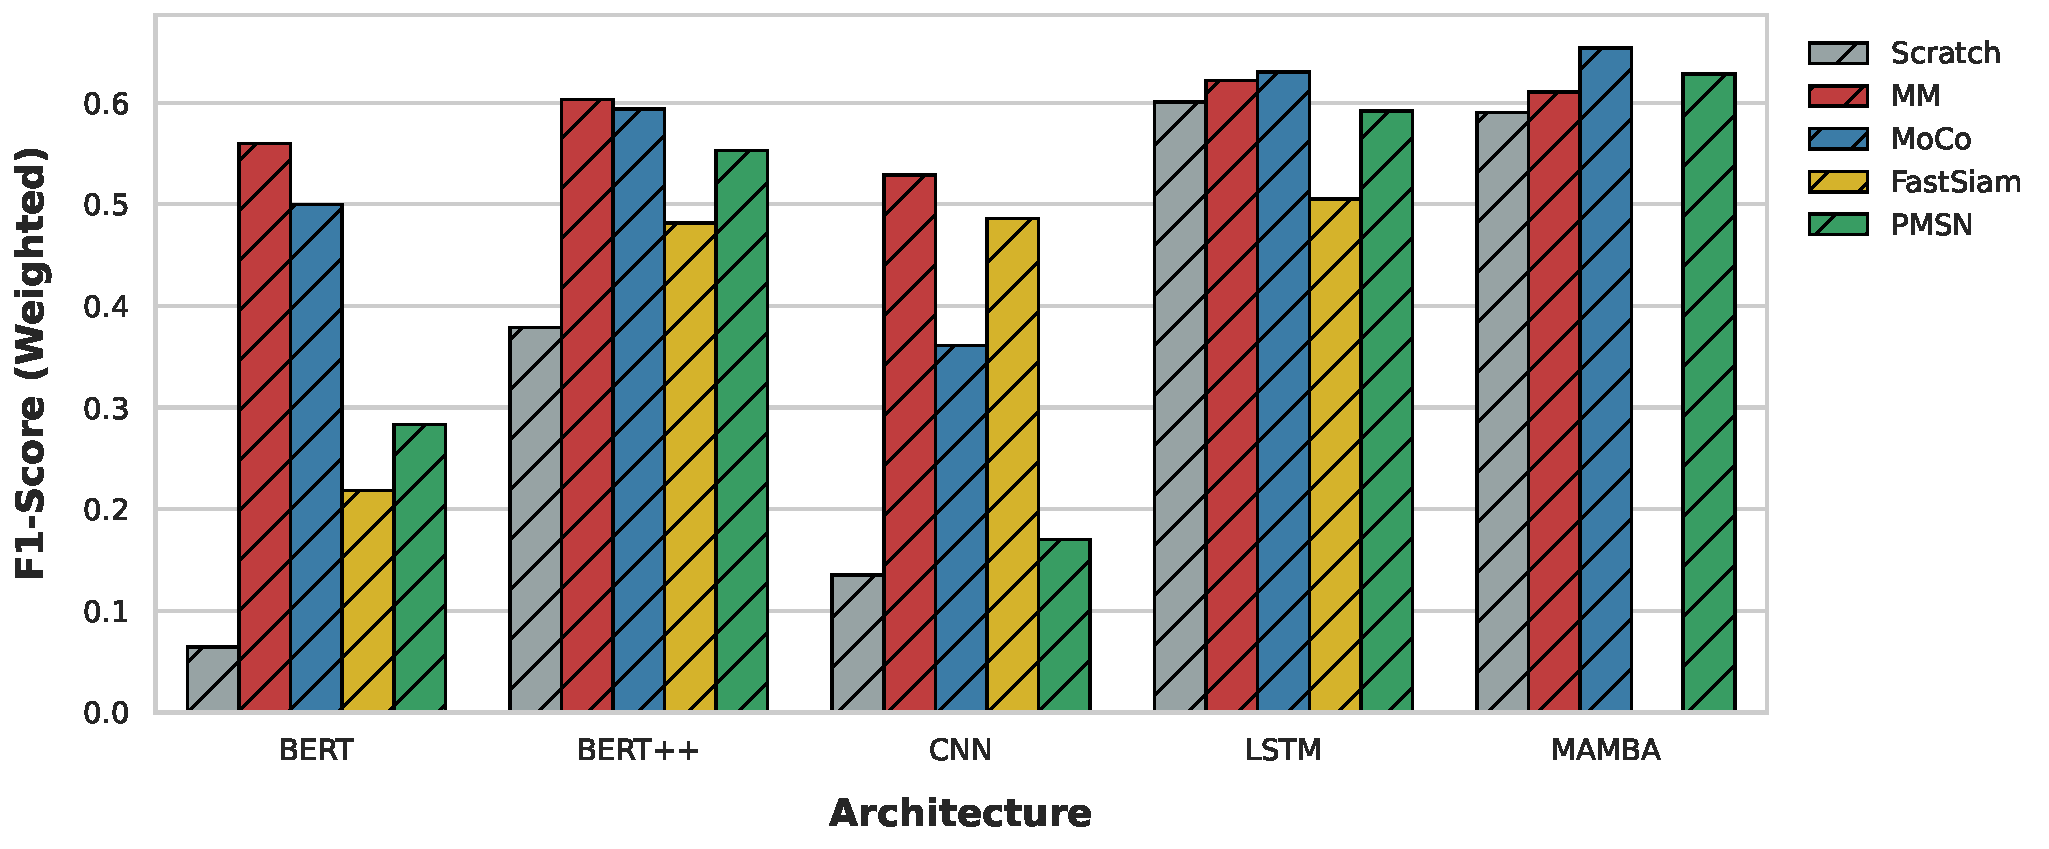
\includegraphics[width=0.7\linewidth]{figures/8_results/brazil-finetuning/few_shot_pretraining.pdf}
    \label{fig:fewshot_finetuning_few_brazil}
\end{figure}

\begin{figure}[ht!]
    \centering
    \caption{F1 Weighted of finetuning model per pretraining in few shot (0.1\% of training data) in California dataset.}
    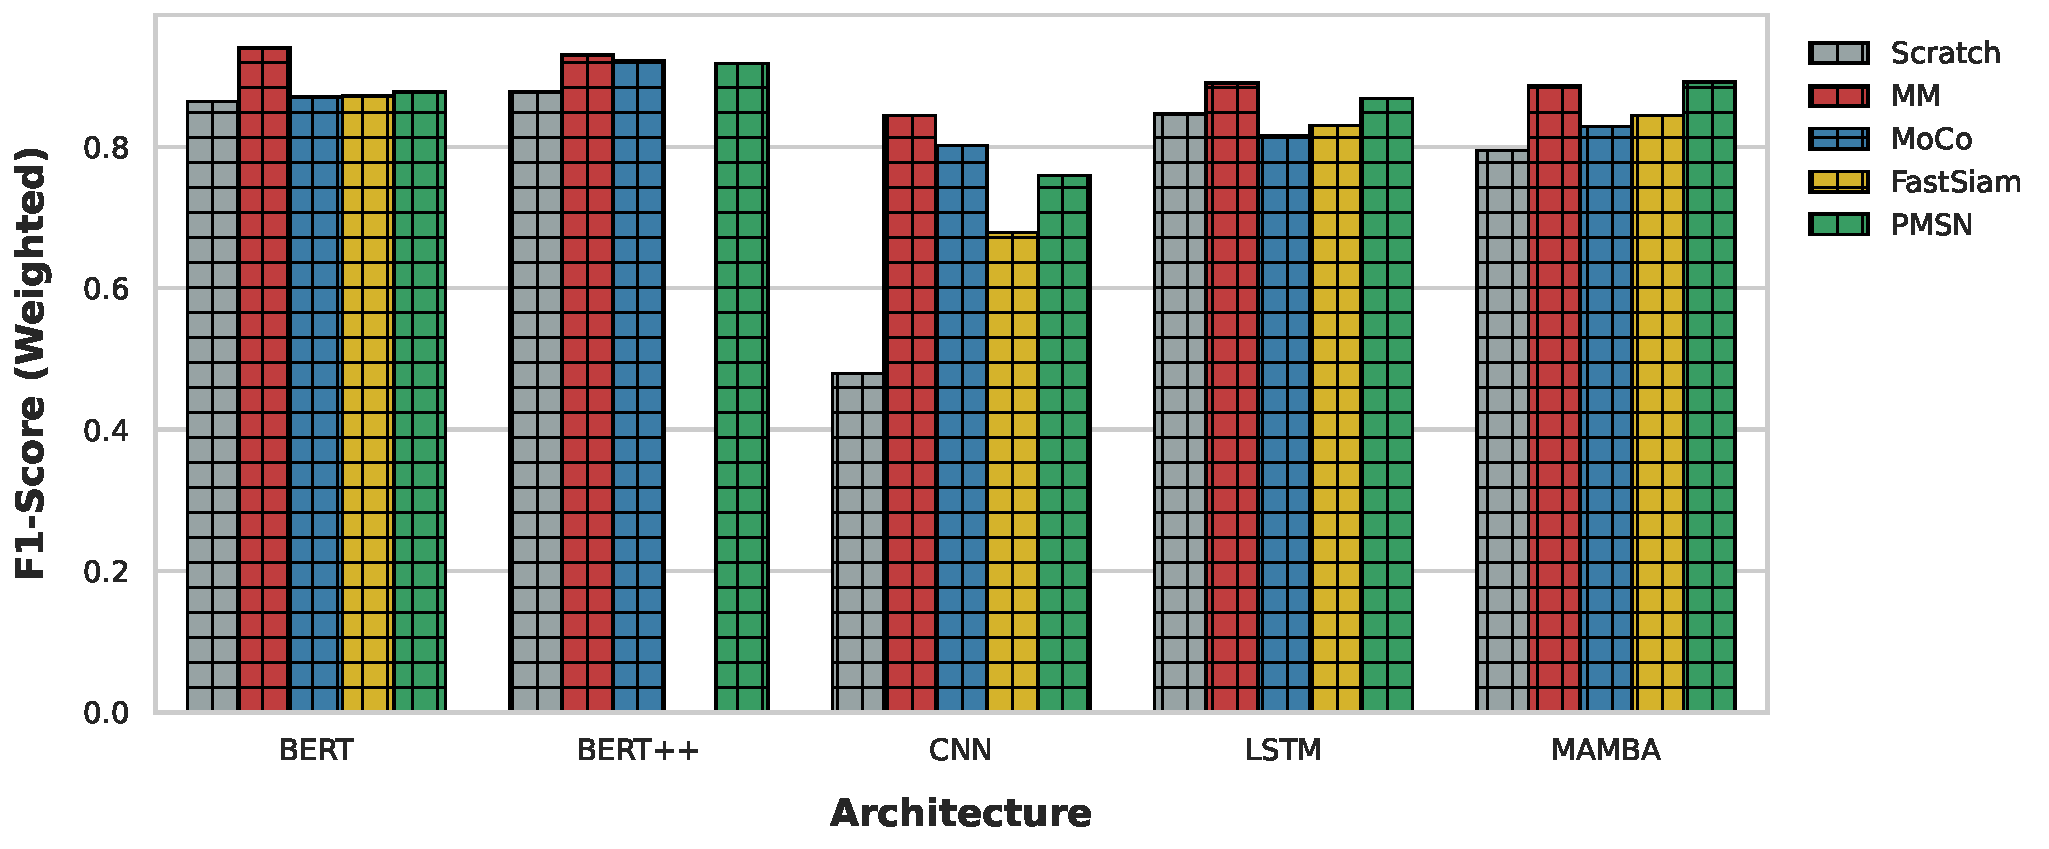
\includegraphics[width=0.7\linewidth]{figures/8_results/california-finetuning/few_shot_pretraining.pdf}
    \label{fig:fewshot_finetuning_few_california}
\end{figure}

\begin{figure}[ht!]
    \centering
    \caption{F1 Weighted of finetuning model per pretraining in few shot (0.1\% of training data) in Texas dataset.}
    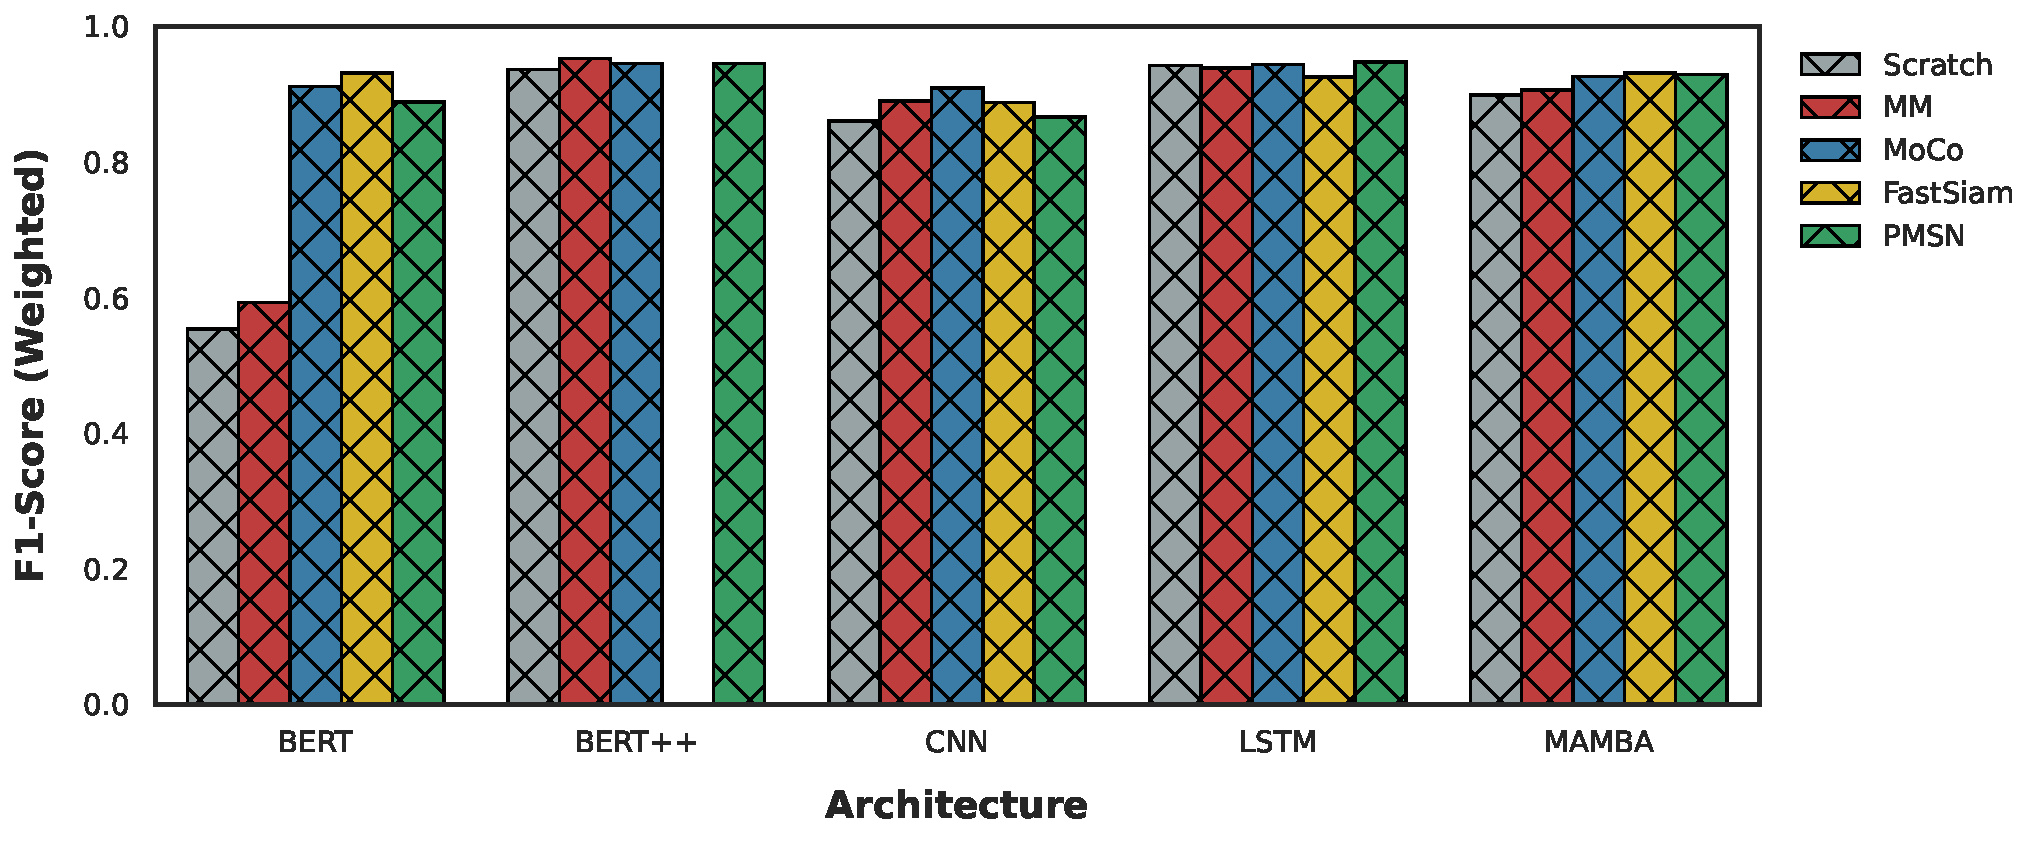
\includegraphics[width=0.7\linewidth]{figures/8_results/texas-finetuning/few_shot_pretraining.pdf}
    \label{fig:fewshot_finetuning_few_texas}
\end{figure}

In Brazil, the impact of pre-training is greater than that of other datasets (see Figure \ref{fig:fewshot_finetuning_few_brazil}). In scenarios with only 1\% of labeled data, models pre-trained with MoCo and MM significantly outperformed their from-scratch versions. SITS-BERT, for example, achieved gains of just over 21\% in F1 Weighted when using MoCo, and up to 40\% also with MoCo in SITS-CNN. These gains confirm that the internal representations learned during the self-supervised phase act as a powerful regularizer, preventing overfitting when labels are scarce. The model starts finetuning with a better initialization than random weights, which is crucial for the complex decision boundaries of the Brazil dataset. In this dataset and scenario, all pre-trainings showed some increase in the metric, with the most marginal being MM for SITS-Mamba, with less than 3\% gain. However, it is important to mention that this model, together with LSTM, already showed high results when compared to the others, even without pre-training.

In the California and Texas datasets (see Figures \ref{fig:fewshot_finetuning_few_california} and \ref{fig:fewshot_finetuning_few_texas}), the advantage of SSL is less noticeable, even in few-shot regimes. However, due to the apparent high separability of classes, even models trained from scratch tend to perform well, with the exceptions of the SITS-CNN models in California and SITS-BERT in Texas.

As for the impact of SSL pre-training on other data regimes, the gains are much smaller, although in very few cases there is a deterioration in performance due to pre-training. The convergence of the curves in Figures \ref{fig:fewshot_finetuning_brazil} through \ref{fig:fewshot_finetuning_texas} as the data percentage increases to 70\% (with enough labeled data), the supervised signal becomes strong enough to learn optimal features directly, rendering the pre-training initialization less critical. In addition, it is noteworthy that some models in some experiments generated unexpected results, indicating a poor fit. SITS-Mamba with MM in Brazil (see Figure \ref{fig:fewshot_finetuning_brazil}) showed a drop in performance when increasing the amount of labeled data from 1\% to 10\%, along with SVM in the same dataset. It is also noteworthy, analyzing the pre-training curves in relation to the shaded area of all datasets (see Figures \ref{fig:fewshot_finetuning_brazil}, \ref{fig:fewshot_finetuning_california}, and \ref{fig:fewshot_finetuning_texas}), that SITS-BERT and SITS-CNN are the models that most depend on pre-training, especially in few-shot scenarios, to present good results.

\begin{figure}[ht!]
    \centering
    \caption{F1 Weighted of finetuning model per pretraining in all data scarcity scenarios in Brazil dataset.}
    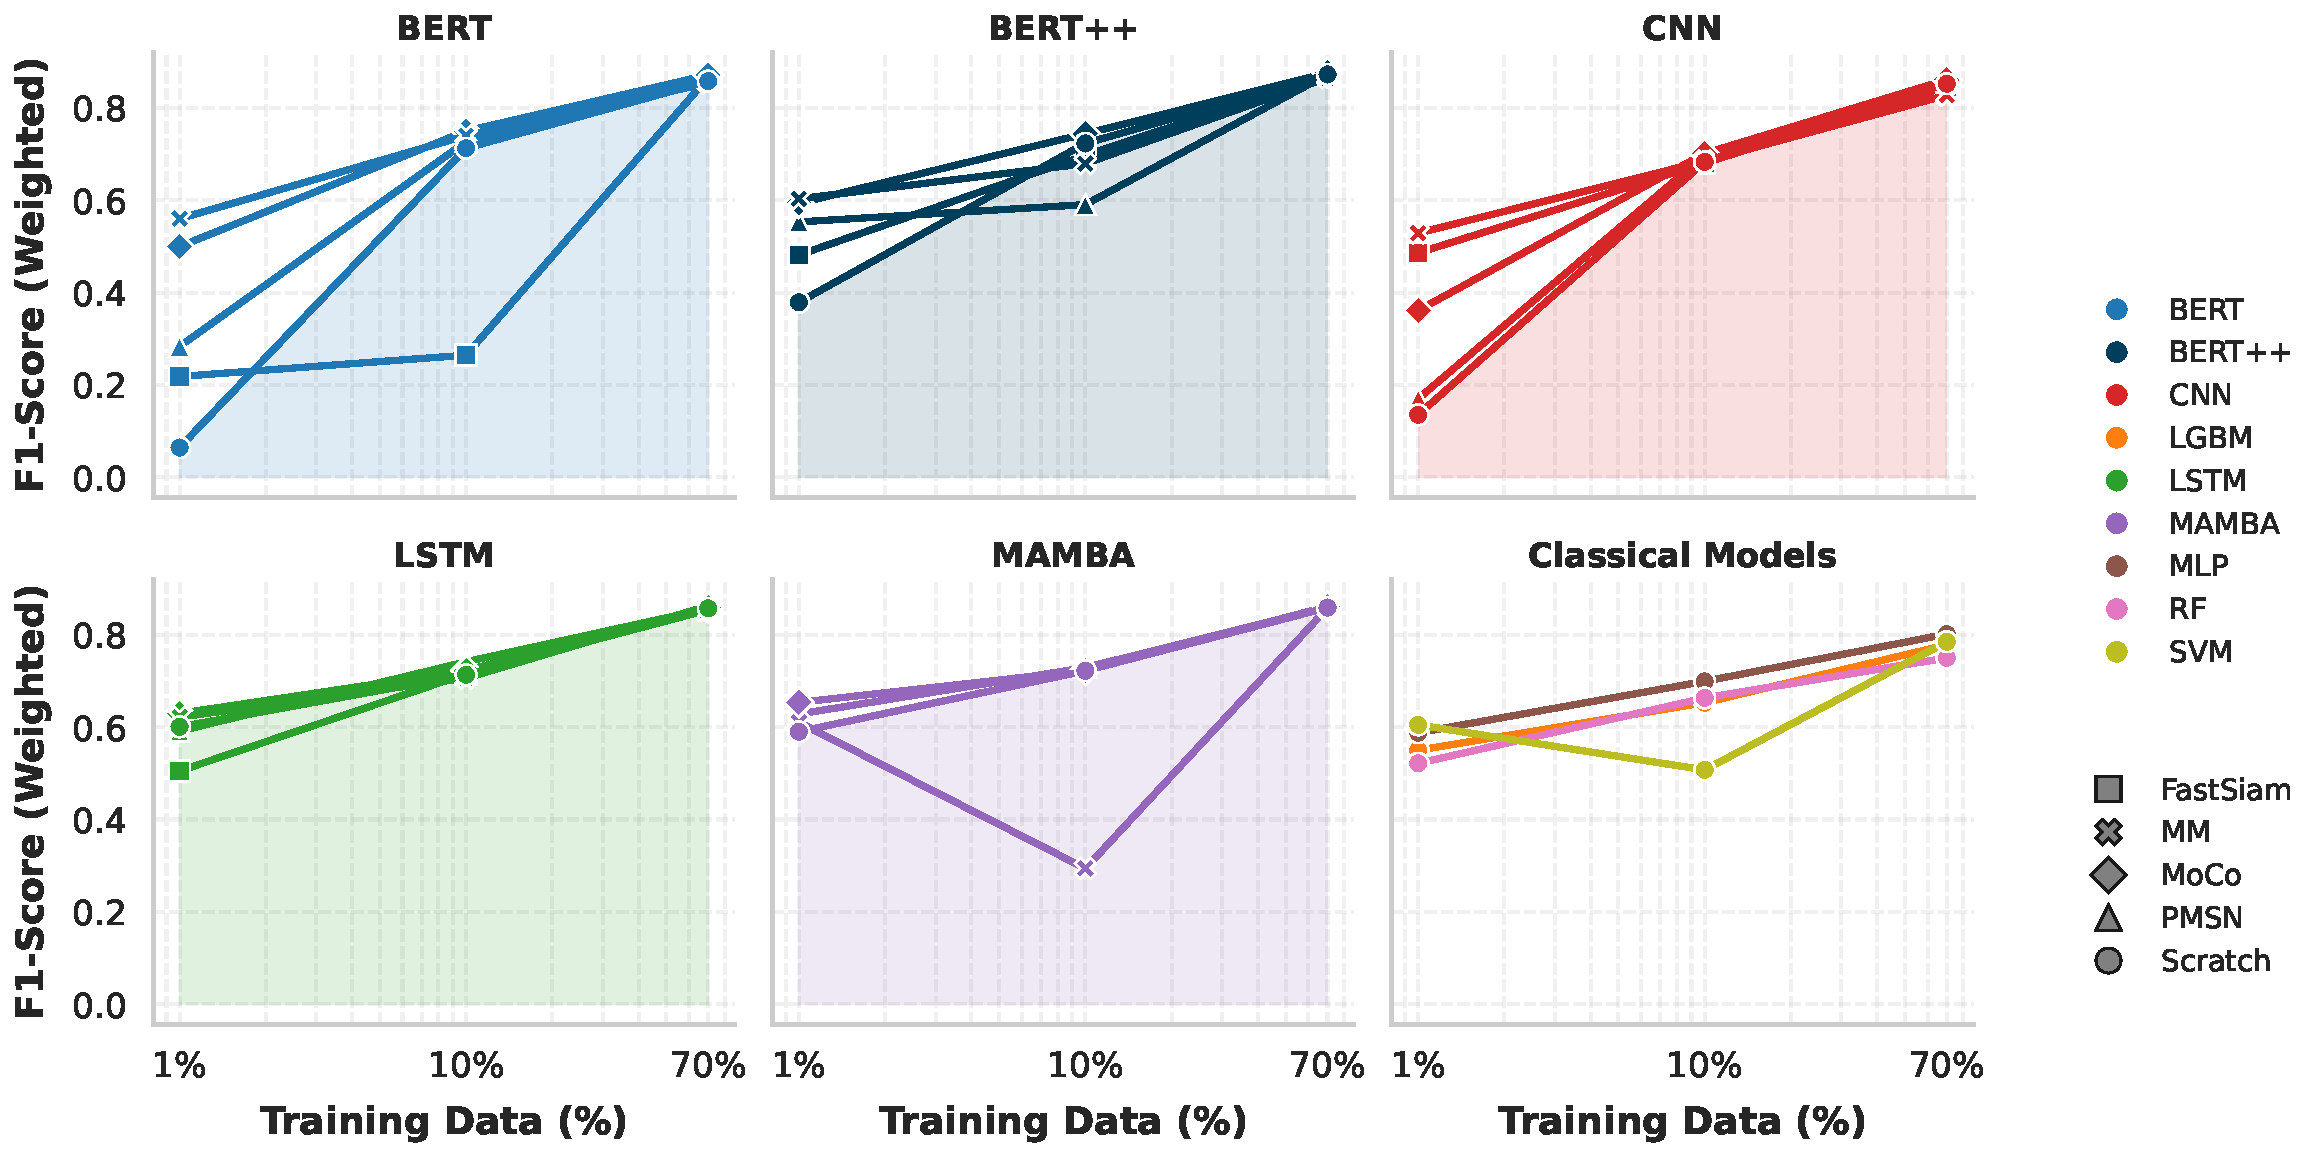
\includegraphics[width=0.7\linewidth]{figures/8_results/brazil-finetuning/line_training.pdf}
    \label{fig:fewshot_finetuning_brazil}
\end{figure}

\begin{figure}[ht!]
    \centering
    \caption{F1 Weighted of finetuning model per pretraining in all data scarcity scenarios in California dataset.}
    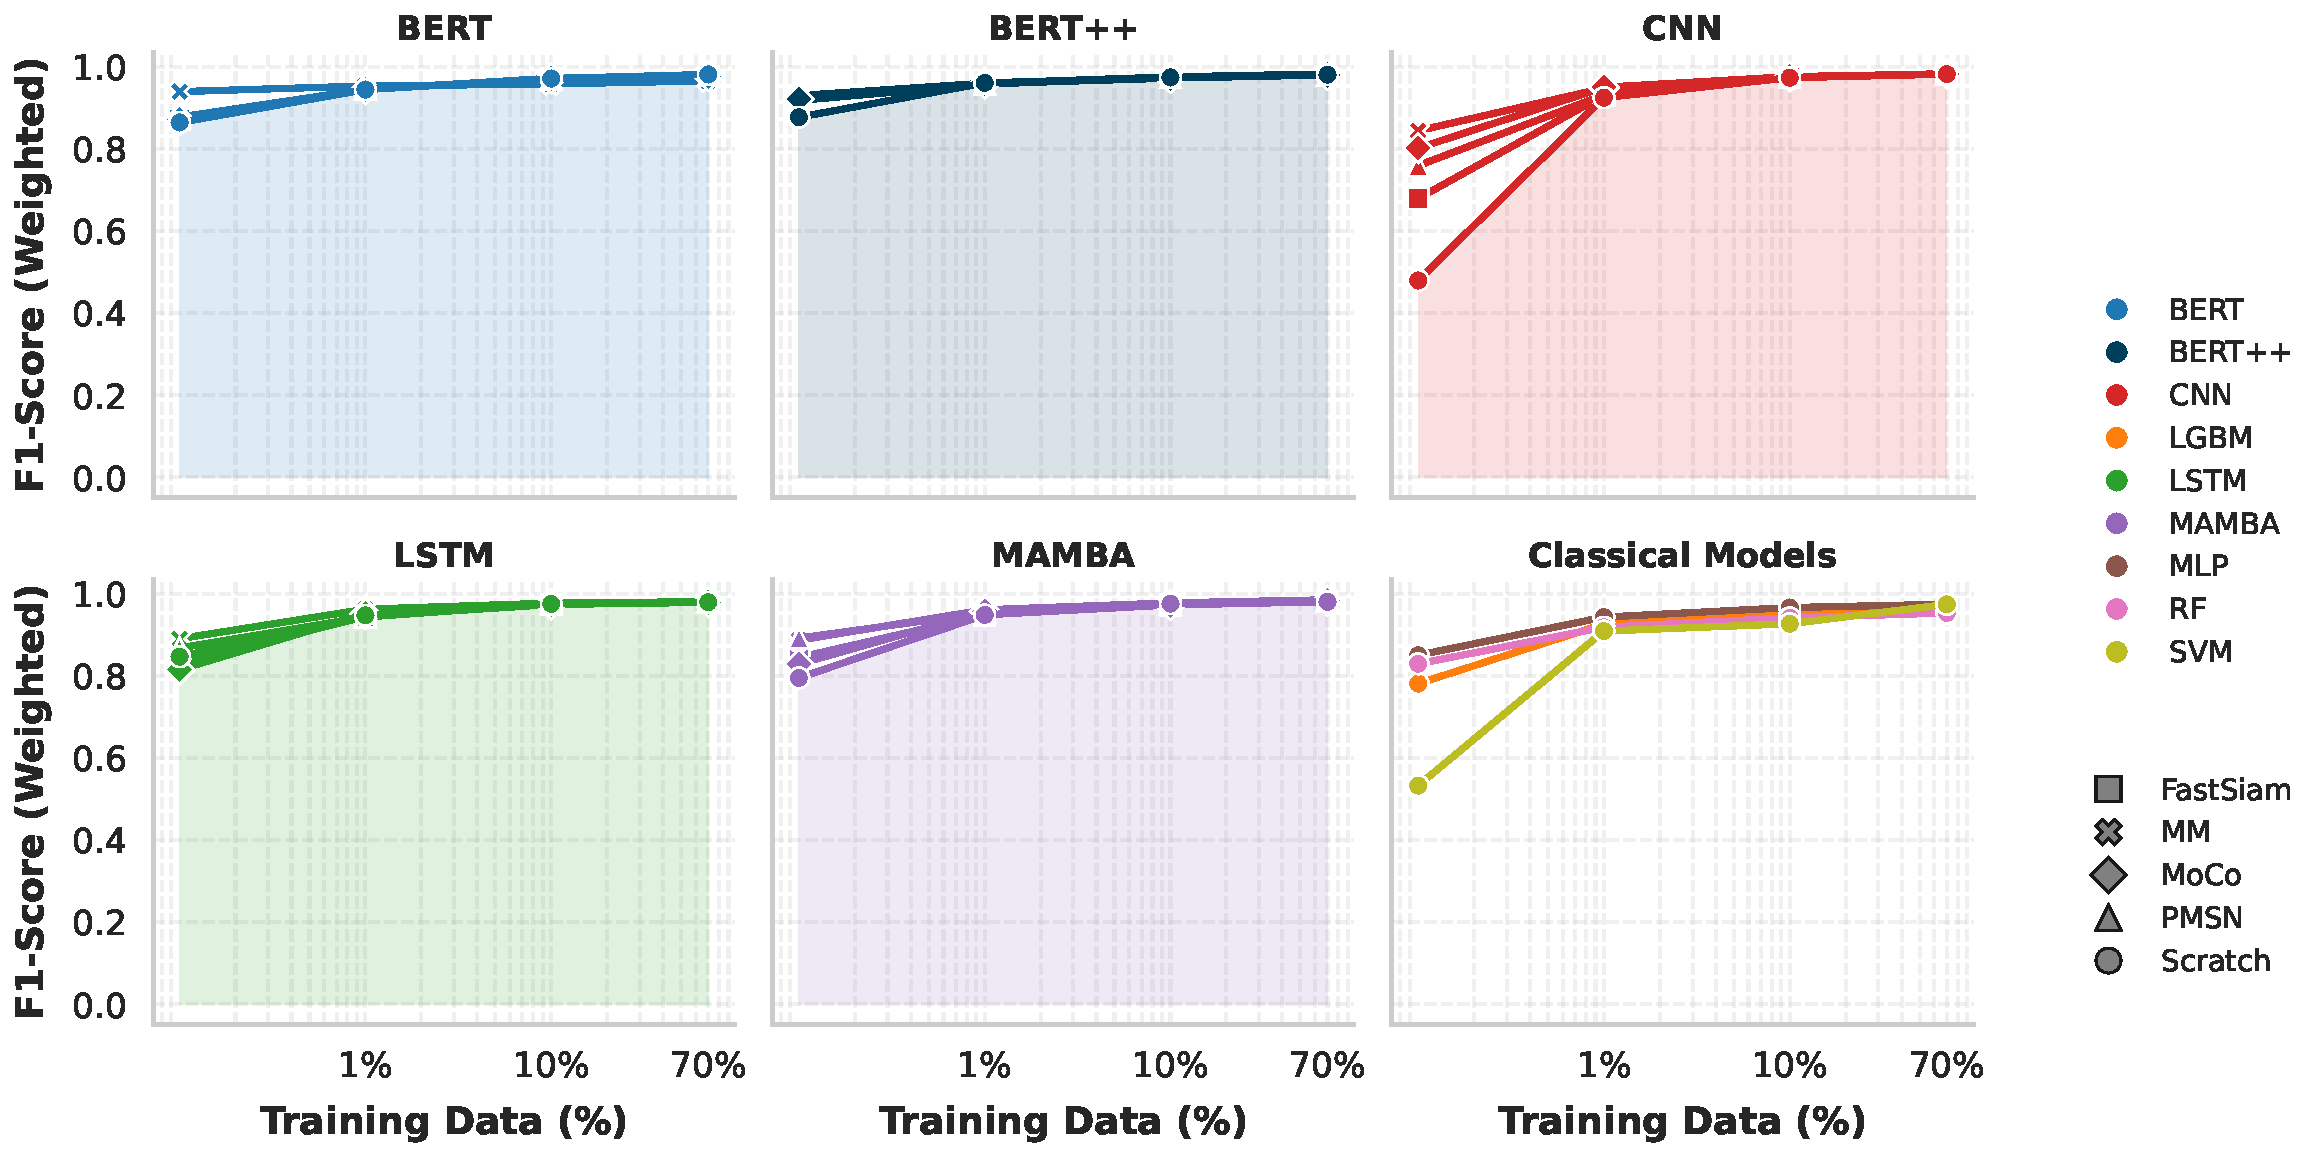
\includegraphics[width=0.7\linewidth]{figures/8_results/california-finetuning/line_training.pdf}
    \label{fig:fewshot_finetuning_california}
\end{figure}

\begin{figure}[ht!]
    \centering
    \caption{F1 Weighted of finetuning model per pretraining in all data scarcity scenarios in Texas dataset.}
    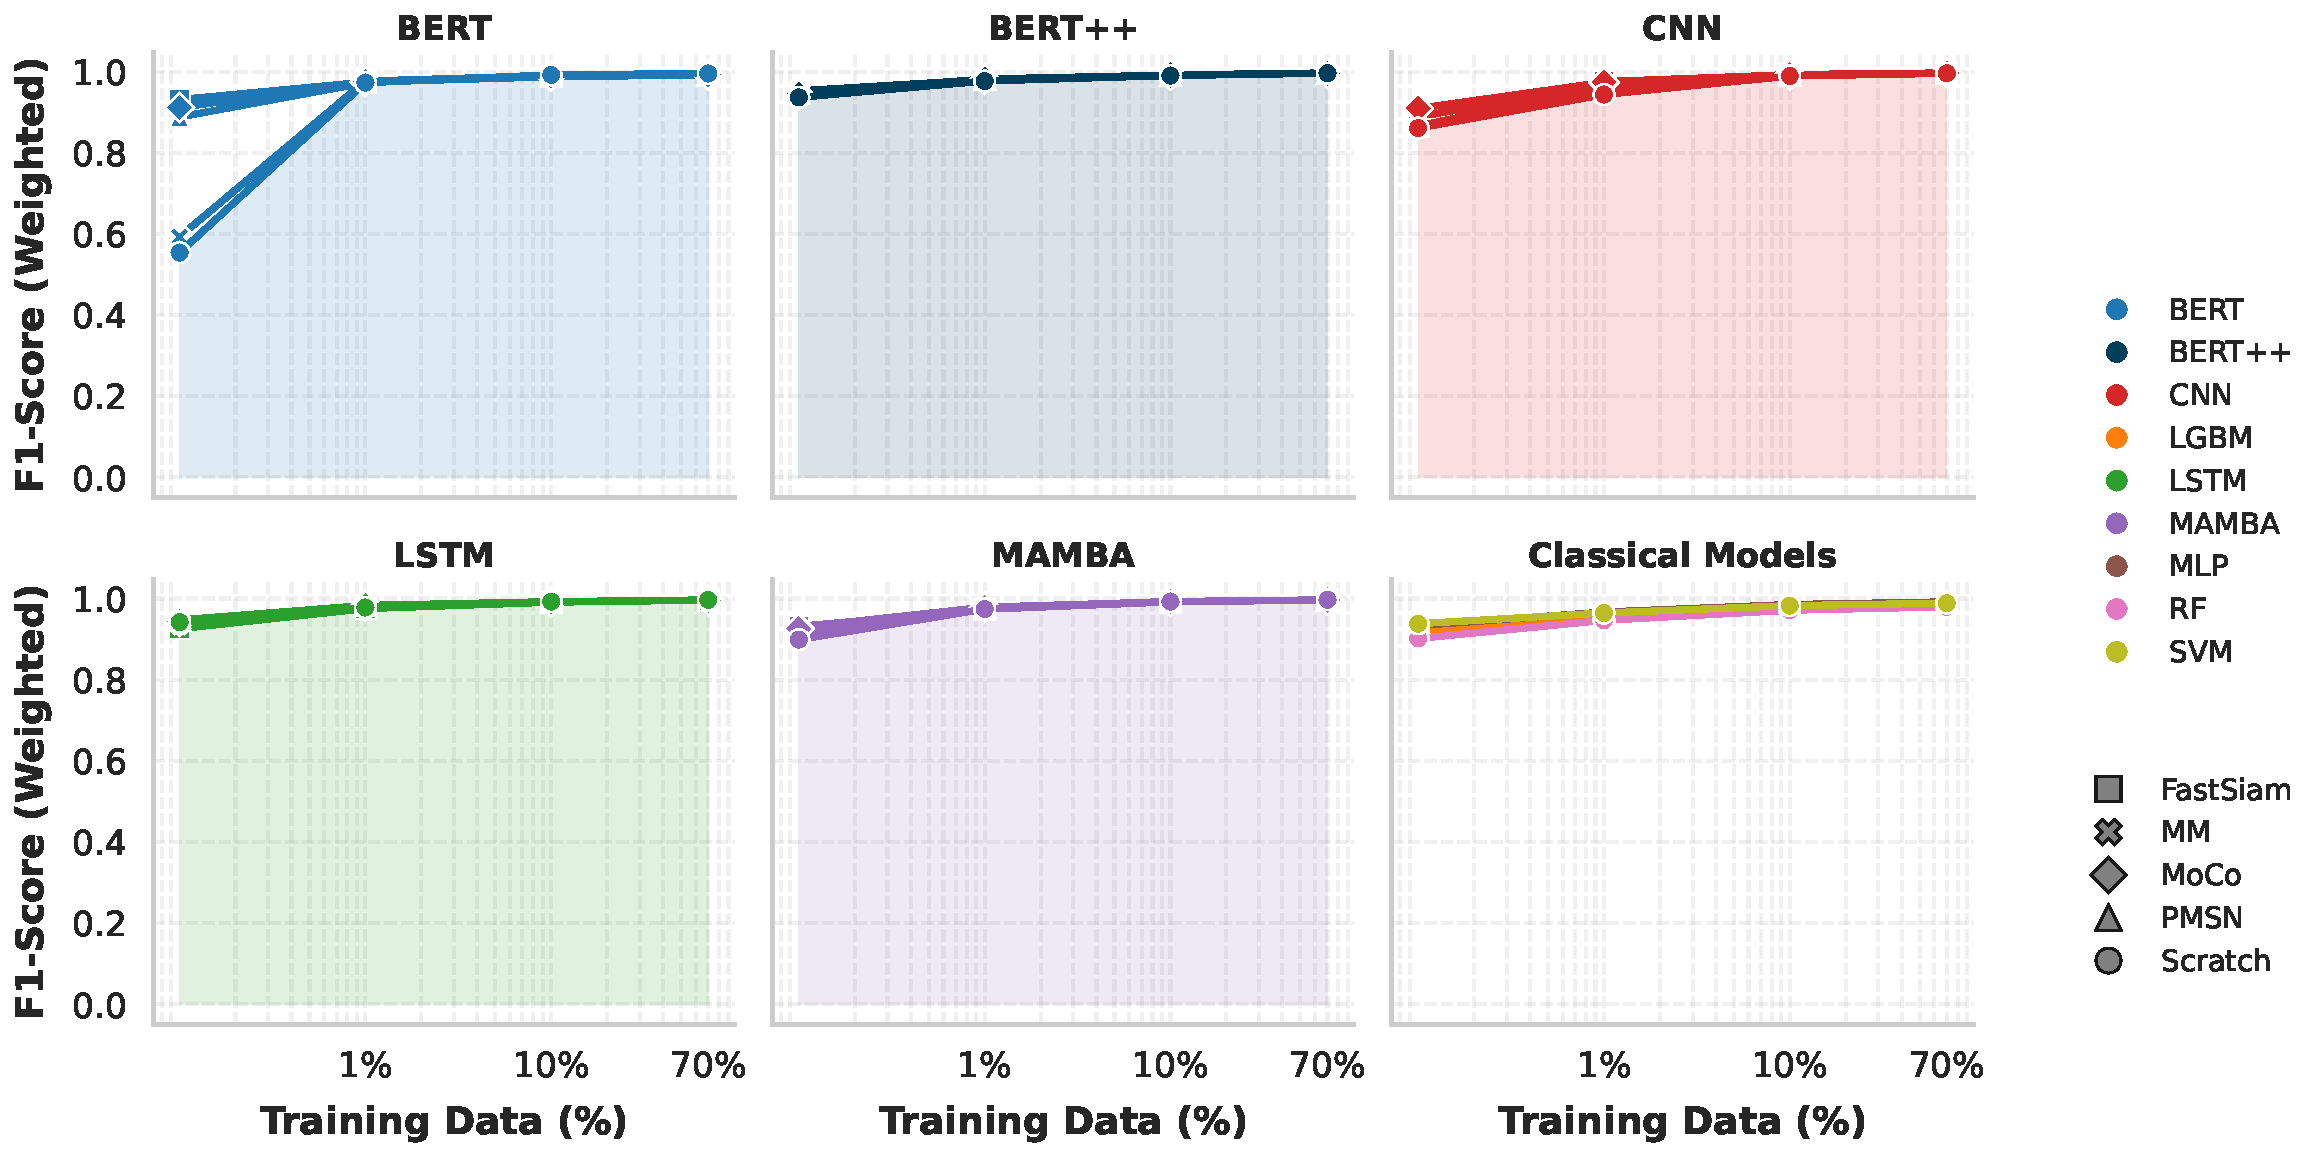
\includegraphics[width=0.7\linewidth]{figures/8_results/texas-finetuning/line_training.pdf}
    \label{fig:fewshot_finetuning_texas}
\end{figure}

\section{ORDER Anomaly Detection}

In the Brazil dataset (see Figure \ref{fig:trust_finetuning_brazil}), removing 5\% to 8\% of samples considered anomalous resulted in a consistent increase in performance (from around 84\% to around 88\% in some models), suggesting that ORDER was effective in identifying samples with noisy labels from Mapbiomas or plots with atypical spectral behavior. Furthermore, it is noticeable that MoCo pre-training identifies a similar number of anomalies even with a low percentage of removed samples when compared to PMSN or from scratch, indicating that the embeddings generated by MoCo are more robust and facilitate the detection of outliers.

\begin{figure}[ht!]
    \centering
    \caption{ORDER per model and pretraining in Brazil dataset.}
    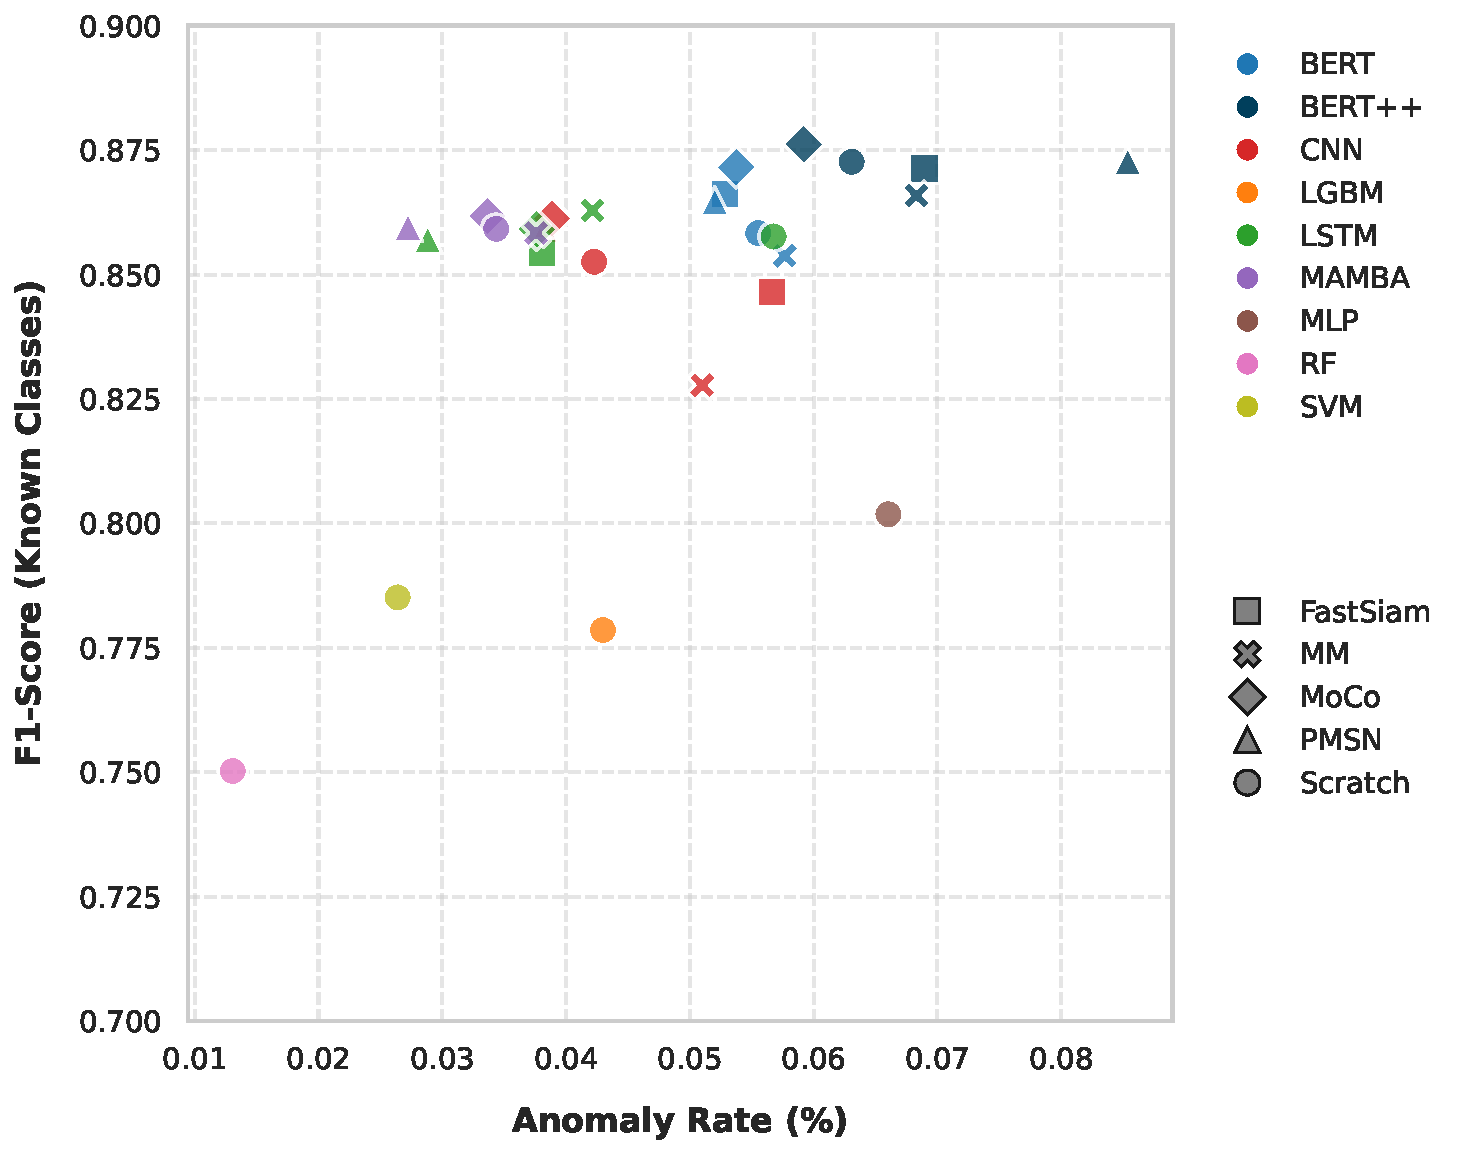
\includegraphics[width=0.6\linewidth]{figures/8_results/brazil-finetuning/trust_analysis.pdf}
    \label{fig:trust_finetuning_brazil}
    \fignote{The Y-axis starts at 0.7 and ends at 0.9.}
\end{figure}

\begin{figure}[ht!]
    \centering
    \caption{ORDER per model and pretraining in California dataset.}
    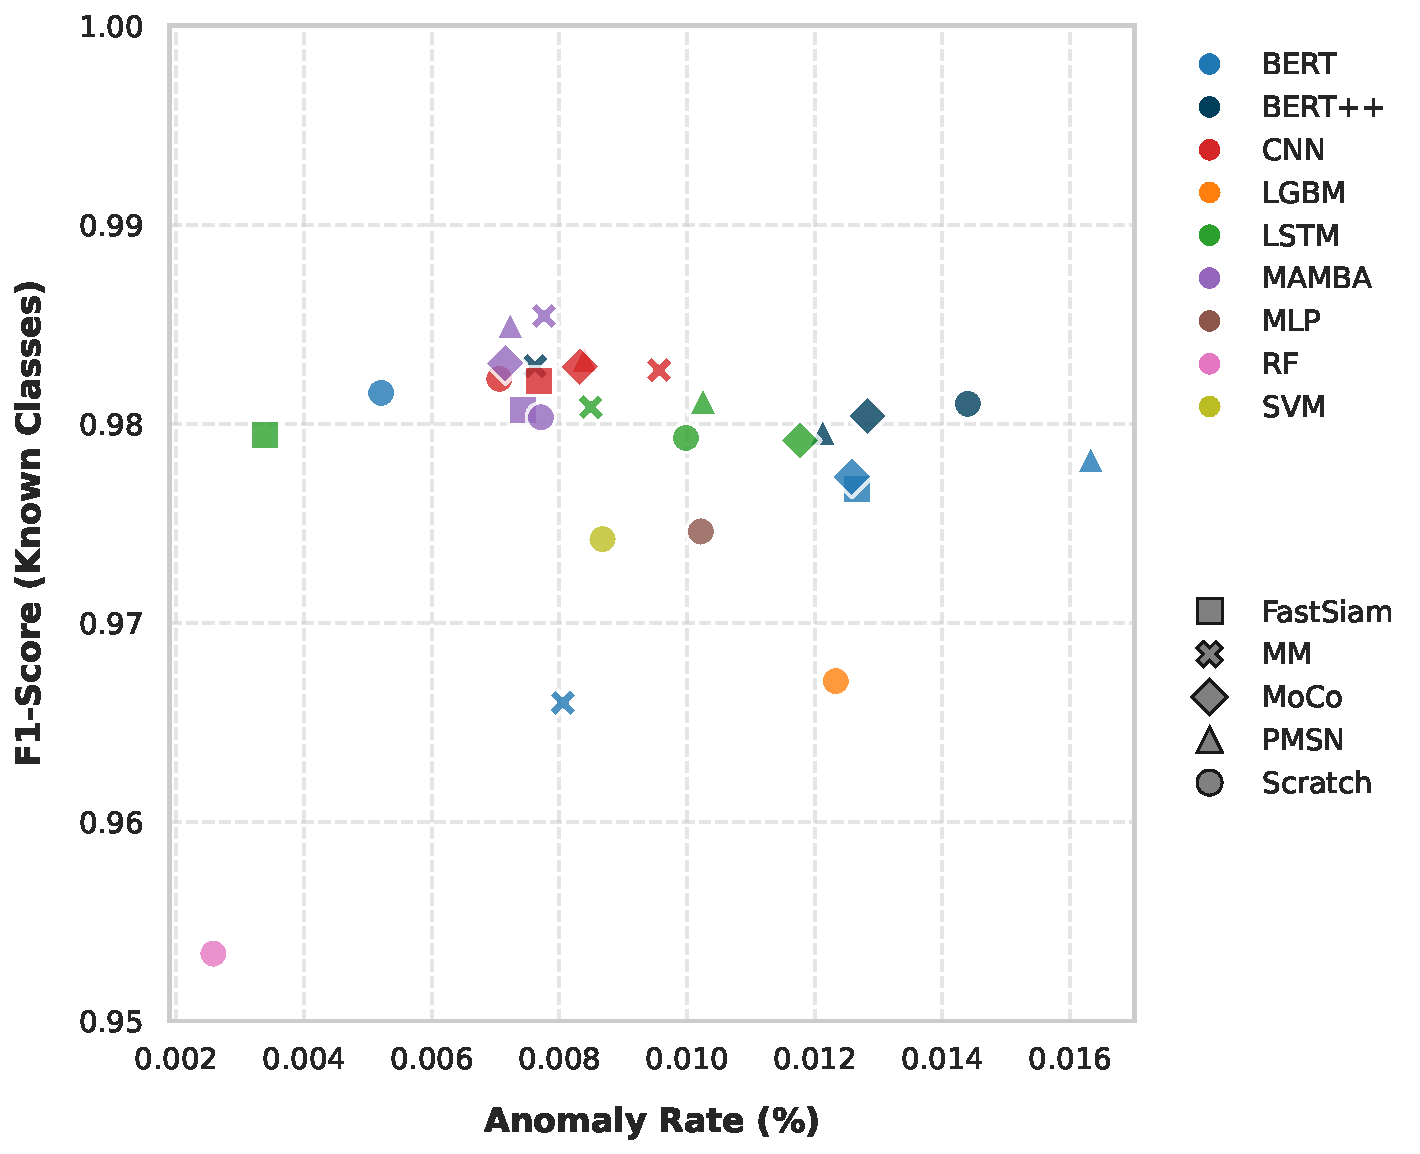
\includegraphics[width=0.6\linewidth]{figures/8_results/california-finetuning/trust_analysis.pdf}
    \label{fig:trust_finetuning_california}
    \fignote{The Y-axis starts at 0.9 and ends at 1.0.}
\end{figure}

\begin{figure}[ht!]
    \centering
    \caption{ORDER per model and pretraining in Texas dataset.}
    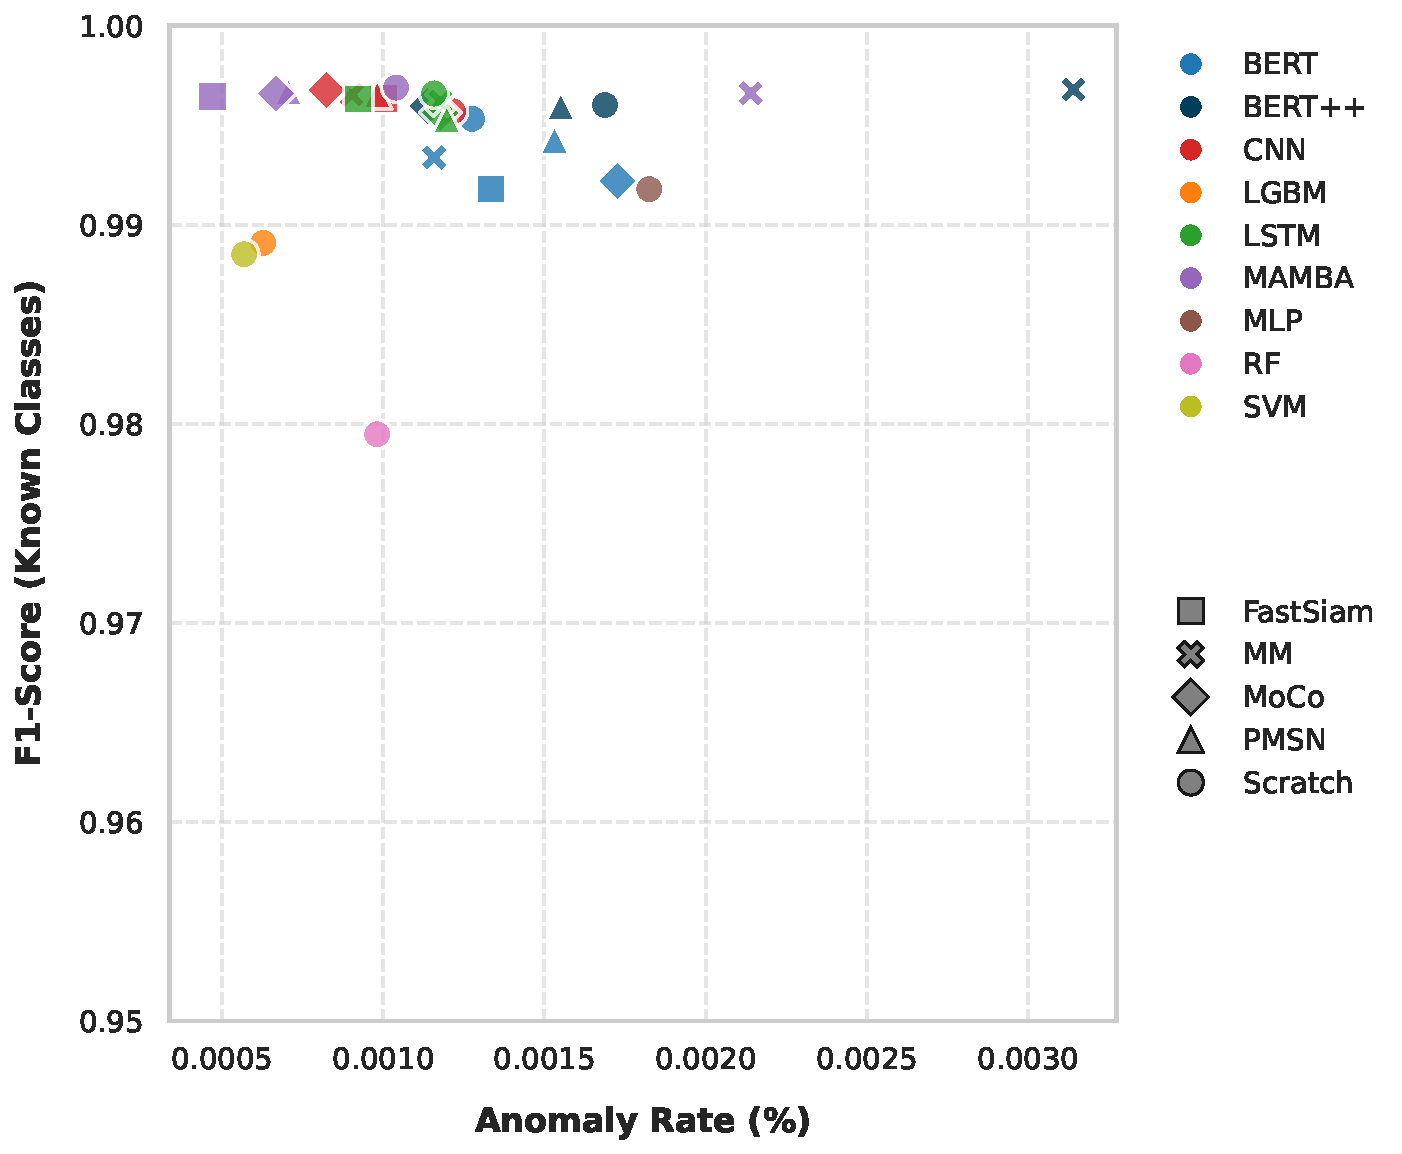
\includegraphics[width=0.6\linewidth]{figures/8_results/texas-finetuning/trust_analysis.pdf}
    \label{fig:trust_finetuning_texas}
    \fignote{The Y-axis starts at 0.9 and ends at 1.0.}
\end{figure}

Conversely, for the California and Texas datasets (see Figures \ref{fig:trust_finetuning_california} and \ref{fig:trust_finetuning_texas}), the improvements were more modest, primarily due to the performance saturation where baseline metrics already exceeded 98\%. However, a crucial finding is the stability of the ORDER framework in these high-accuracy regimes. Unlike traditional uncertainty filtering, which often degrades performance in well-separated data by discarding informative hard samples, ORDER maintained metric stability or provided marginal gains. This behavior indicates that the method is selective and conservative, targeting genuine label noise rather than merely removing difficult examples, essentially acting as a safe filter that preserves the decision boundary integrity even when the anomaly rate is naturally low.

\section{Best results per dataset}

This section details the best experiment obtained for each dataset, analyzing the confusion matrices, the distribution of embeddings using t-SNE dimensionality reduction, and verifying the separability between correct and incorrect predictions using the model itself, ConfidNet, and the proposed ORDER method.

\subsection{Brazil Dataset}

\begin{figure}[ht!]
    \centering
    % Início da primeira subfigura (Matriz)
    \begin{subfigure}[b]{0.48\textwidth}
        \centering
        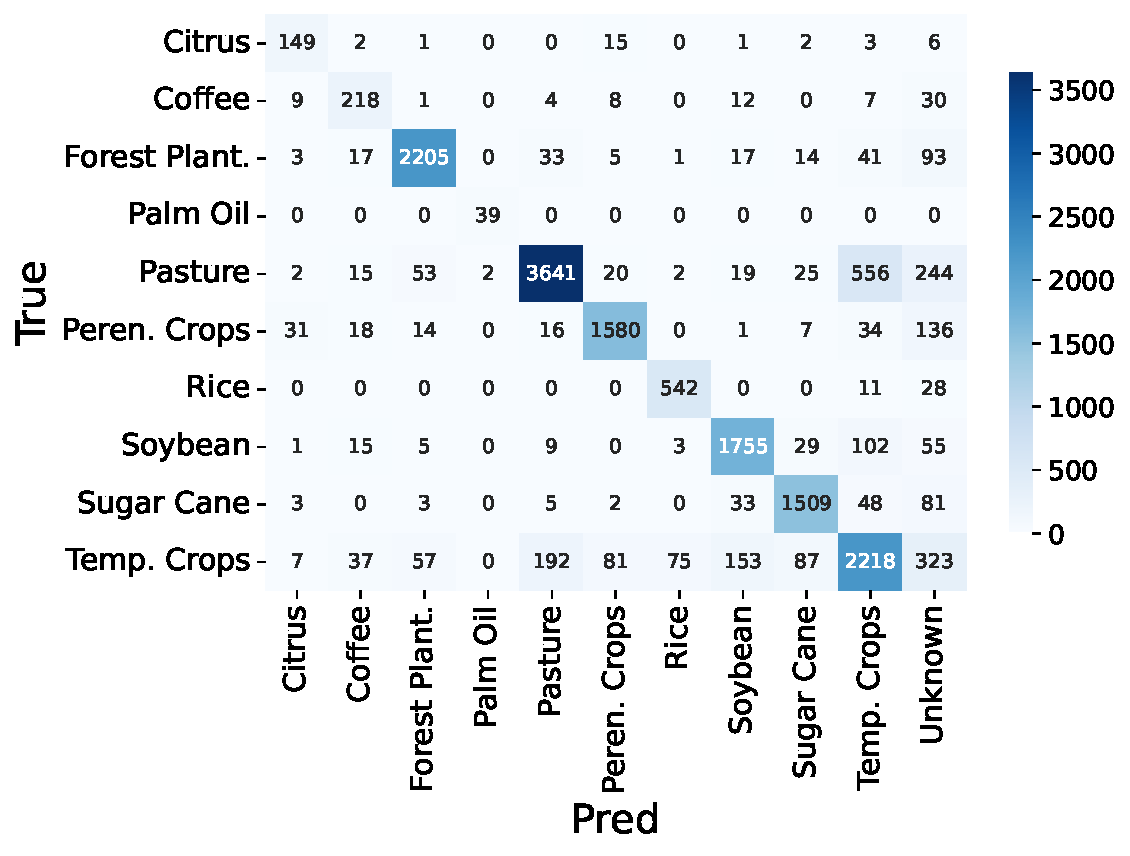
\includegraphics[width=\linewidth]{figures/8_results/brazil-finetuning/BERTPP-70.0-MoCo/class_test_gemmos_matrix.pdf}
        %\caption{Matriz de Confusão}
        \label{fig:brazil_cm}
    \end{subfigure}
    \hfill % Adiciona espaço elástico entre as figuras
    % Início da segunda subfigura (Relatório)
    \begin{subfigure}[b]{0.48\textwidth}
        \centering
        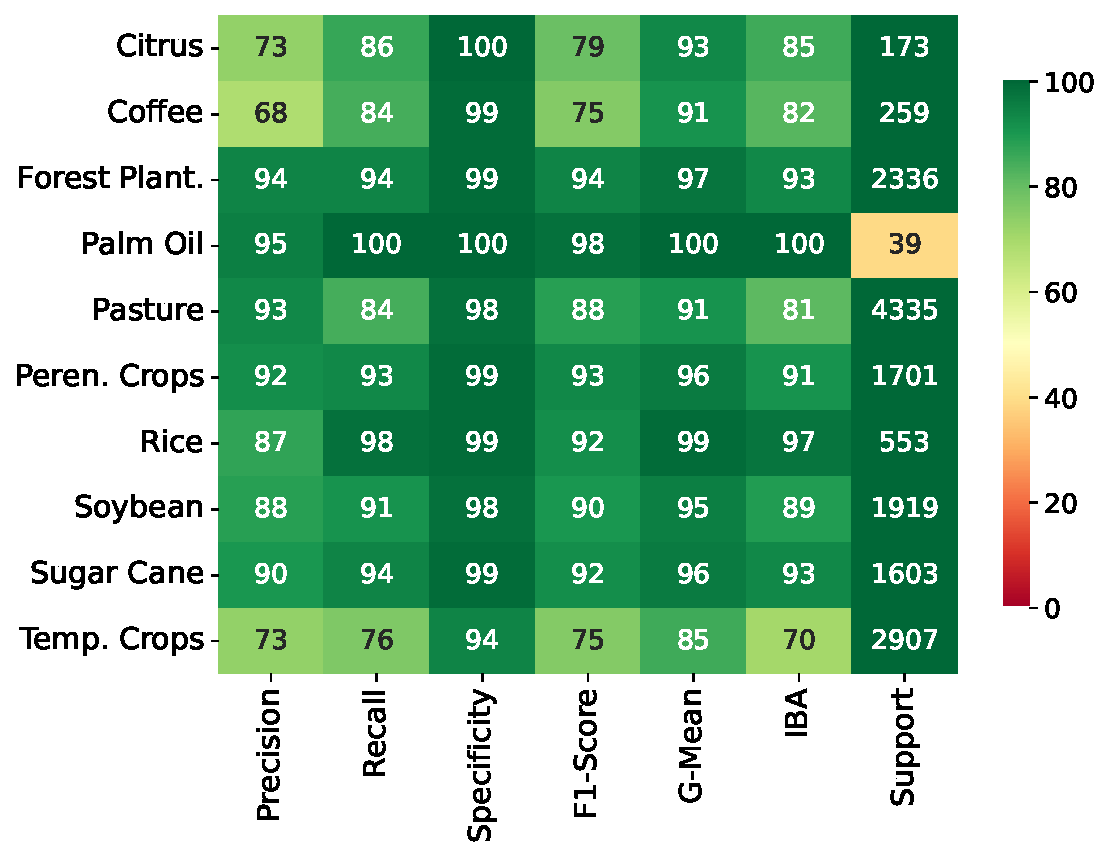
\includegraphics[width=\linewidth]{figures/8_results/brazil-finetuning/BERTPP-70.0-MoCo/class_test_gemmos_report.pdf}
        %\caption{Relatório de Classificação}
        \label{fig:brazil_cr}
    \end{subfigure}
    
    % Legenda geral para ambas as figuras
    \caption{Best experiment in Brazil Dataset class. Report with 70\% in training data (BERT++ with MoCo pretraining).}
    \label{fig:brazil_experiments}
\end{figure}

A closer look of the results from the best experiment on the Brazilian (see \autoref{fig:brazil_experiments}) dataset reveals that the confusion matrix has a significantly high main diagonal, indicating that the model has a high accuracy rate in correctly classifying the classes. The most problematic classes are Pasture, Temporary Crops, and Perennial Crops. The Pasture class is quite complex due to seasonal variations and different agricultural practices that affect its appearance in the SITS, in addition to being more affected by rainfall. The Temporary Crops and Perennial Crops classes, in turn, can contain a variety of crops with different growth cycles, which can lead to classification confusion, and may even include other classes present in the dataset. The \ac{ORDER} method rejects more true samples precisely in these classes, indicating its effectiveness, even in a scenario of high model metrics, where the ConfidNet baseline tends not to perform well.

The evaluation metrics in the classification report confirm the robustness of the framework, with Specificity and G-Mean metrics exceeding 90\% for most categories. However, the Other Temporary Crops and Other Perennial Crops classes show the lowest IBA indices (70 and 91, respectively) and slightly reduced F1-Score metrics when compared to more stable classes, such as Palm Oil and Rice.

\begin{figure}[ht!]
    \centering
    \caption{Best experiment in Brazil Dataset with 70\% in training data (BERT++ with MoCo pretraining) separability between right and wrong predictions with ORDER, ConfidNet and MCP.}
    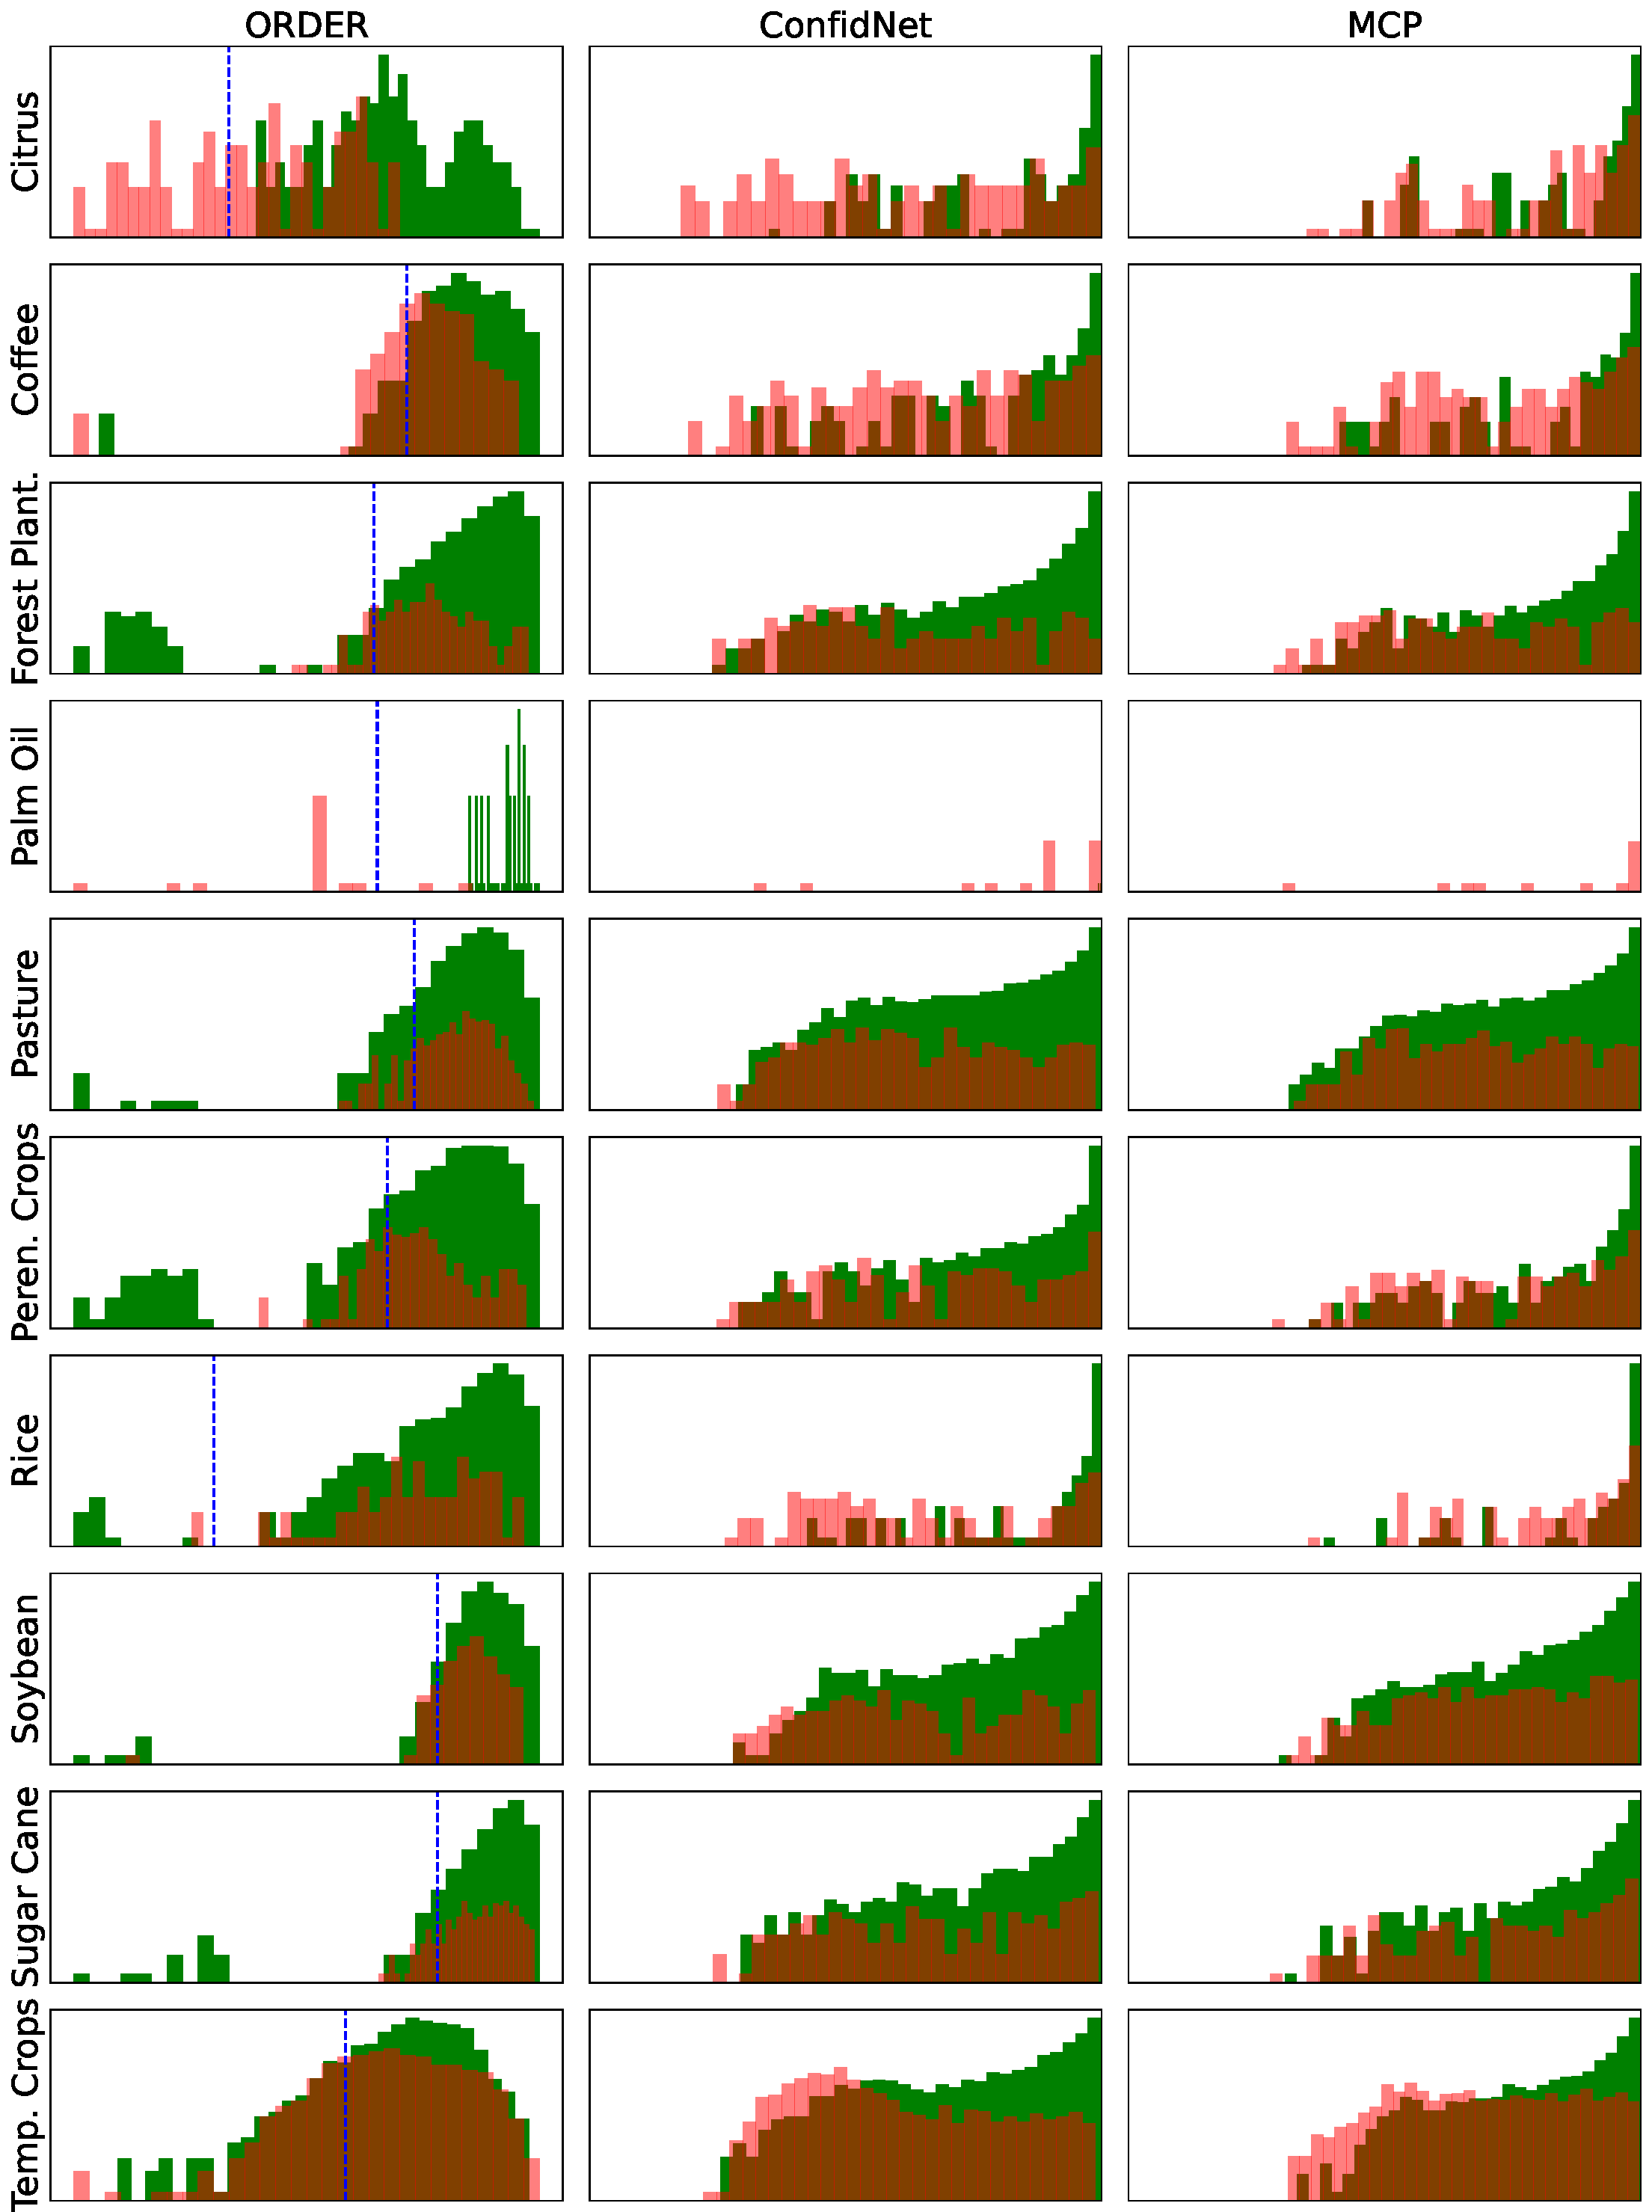
\includegraphics[width=0.6\linewidth]{figures/8_results/brazil-finetuning/BERTPP-70.0-MoCo/hist_combined_test.pdf}
    \label{fig:brazil_gmm}
    \fignote{Y-axis is in logarithmic scale.}
\end{figure}

The histograms illustrate the superiority of ORDER in separating correct from incorrect predictions (see \autoref{fig:brazil_gmm}). While ConfidNet and the Model Confidence show overlapping distributions (Right and Wrong predictions both clustering near high confidence values, being overconfident), the \ac{ORDER} method exhibits a clearer bimodal separation. This separation allows for a more effective thresholding strategy to filter out potential errors without discarding too many correct predictions.

\subsection{Texas Dataset}

\begin{figure}[ht!]
    \centering
    % Início da primeira subfigura (Matriz)
    \begin{subfigure}[b]{0.48\textwidth}
        \centering
        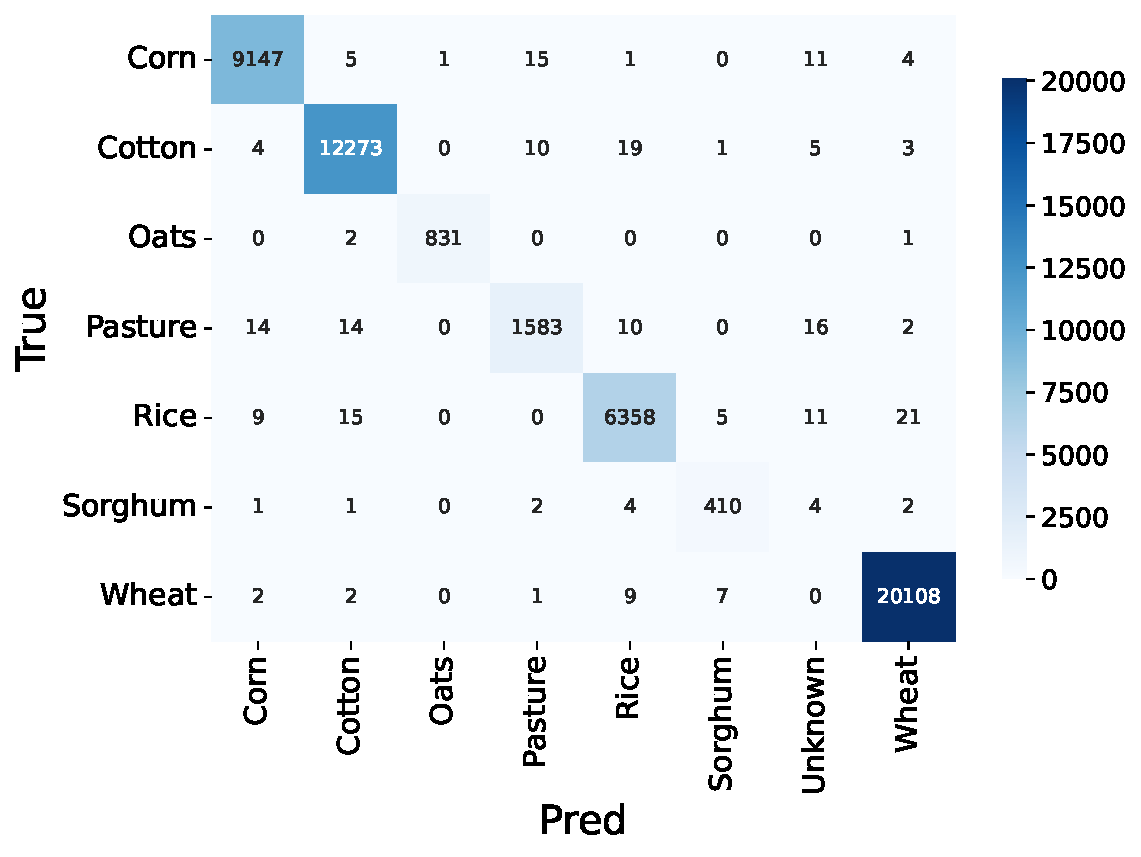
\includegraphics[width=\linewidth]{figures/8_results/texas-finetuning/LSTM-70.0-FastSiam/class_test_gemmos_matrix.pdf}
        %\caption{Matriz de Confusão}
        \label{fig:texas_cm}
    \end{subfigure}
    \hfill % Adiciona espaço elástico entre as figuras
    % Início da segunda subfigura (Relatório)
    \begin{subfigure}[b]{0.48\textwidth}
        \centering
        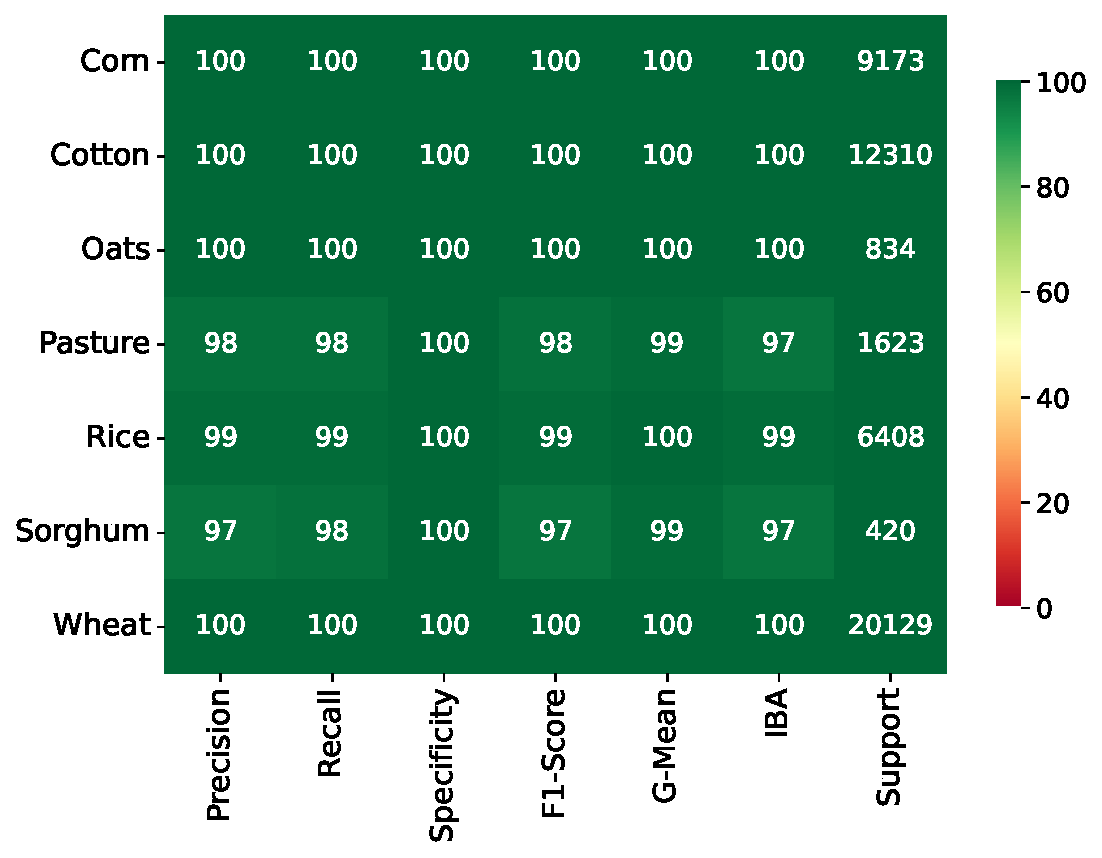
\includegraphics[width=\linewidth]{figures/8_results/texas-finetuning/LSTM-70.0-FastSiam/class_test_gemmos_report.pdf}
        %\caption{Relatório de Classificação}
        \label{fig:texas_cr}
    \end{subfigure}
    
    % Legenda geral para ambas as figuras
    \caption{Best experiment in Texas Dataset with 70\% in training data (LSTM with FastSiam pretraining).}
    \label{fig:texas_experiments}
\end{figure}

Doing the same with the Texas dataset (see \autoref{fig:texas_experiments}), the best experiment on this dataset was using the LSTM model with FastSiam pretraining, revealing  high performance. The confusion matrix shows an extremely clean main diagonal, indicating that the model achieved near-perfect separation for classes such as Corn, Cotton, and Wheat, with hits exceeding 9,000, 12,000, and 20,000 instances, respectively. The reduced incidence of values in the ``Unknown'' column suggests that, in this dataset, the ORDER method found fewer anomalies, which may be attributed to a database with less noisy labels or to a greater spectral-temporal distinction between Texas agricultural crops compared to Brazilian ones.

\begin{figure}[ht!]
    \centering
    \caption{Best experiment in Texas Dataset with 70\% in training data (LSTM with FastSiam pretraining) separability between right and wrong predictions with ORDER, ConfidNet and MCP.}
    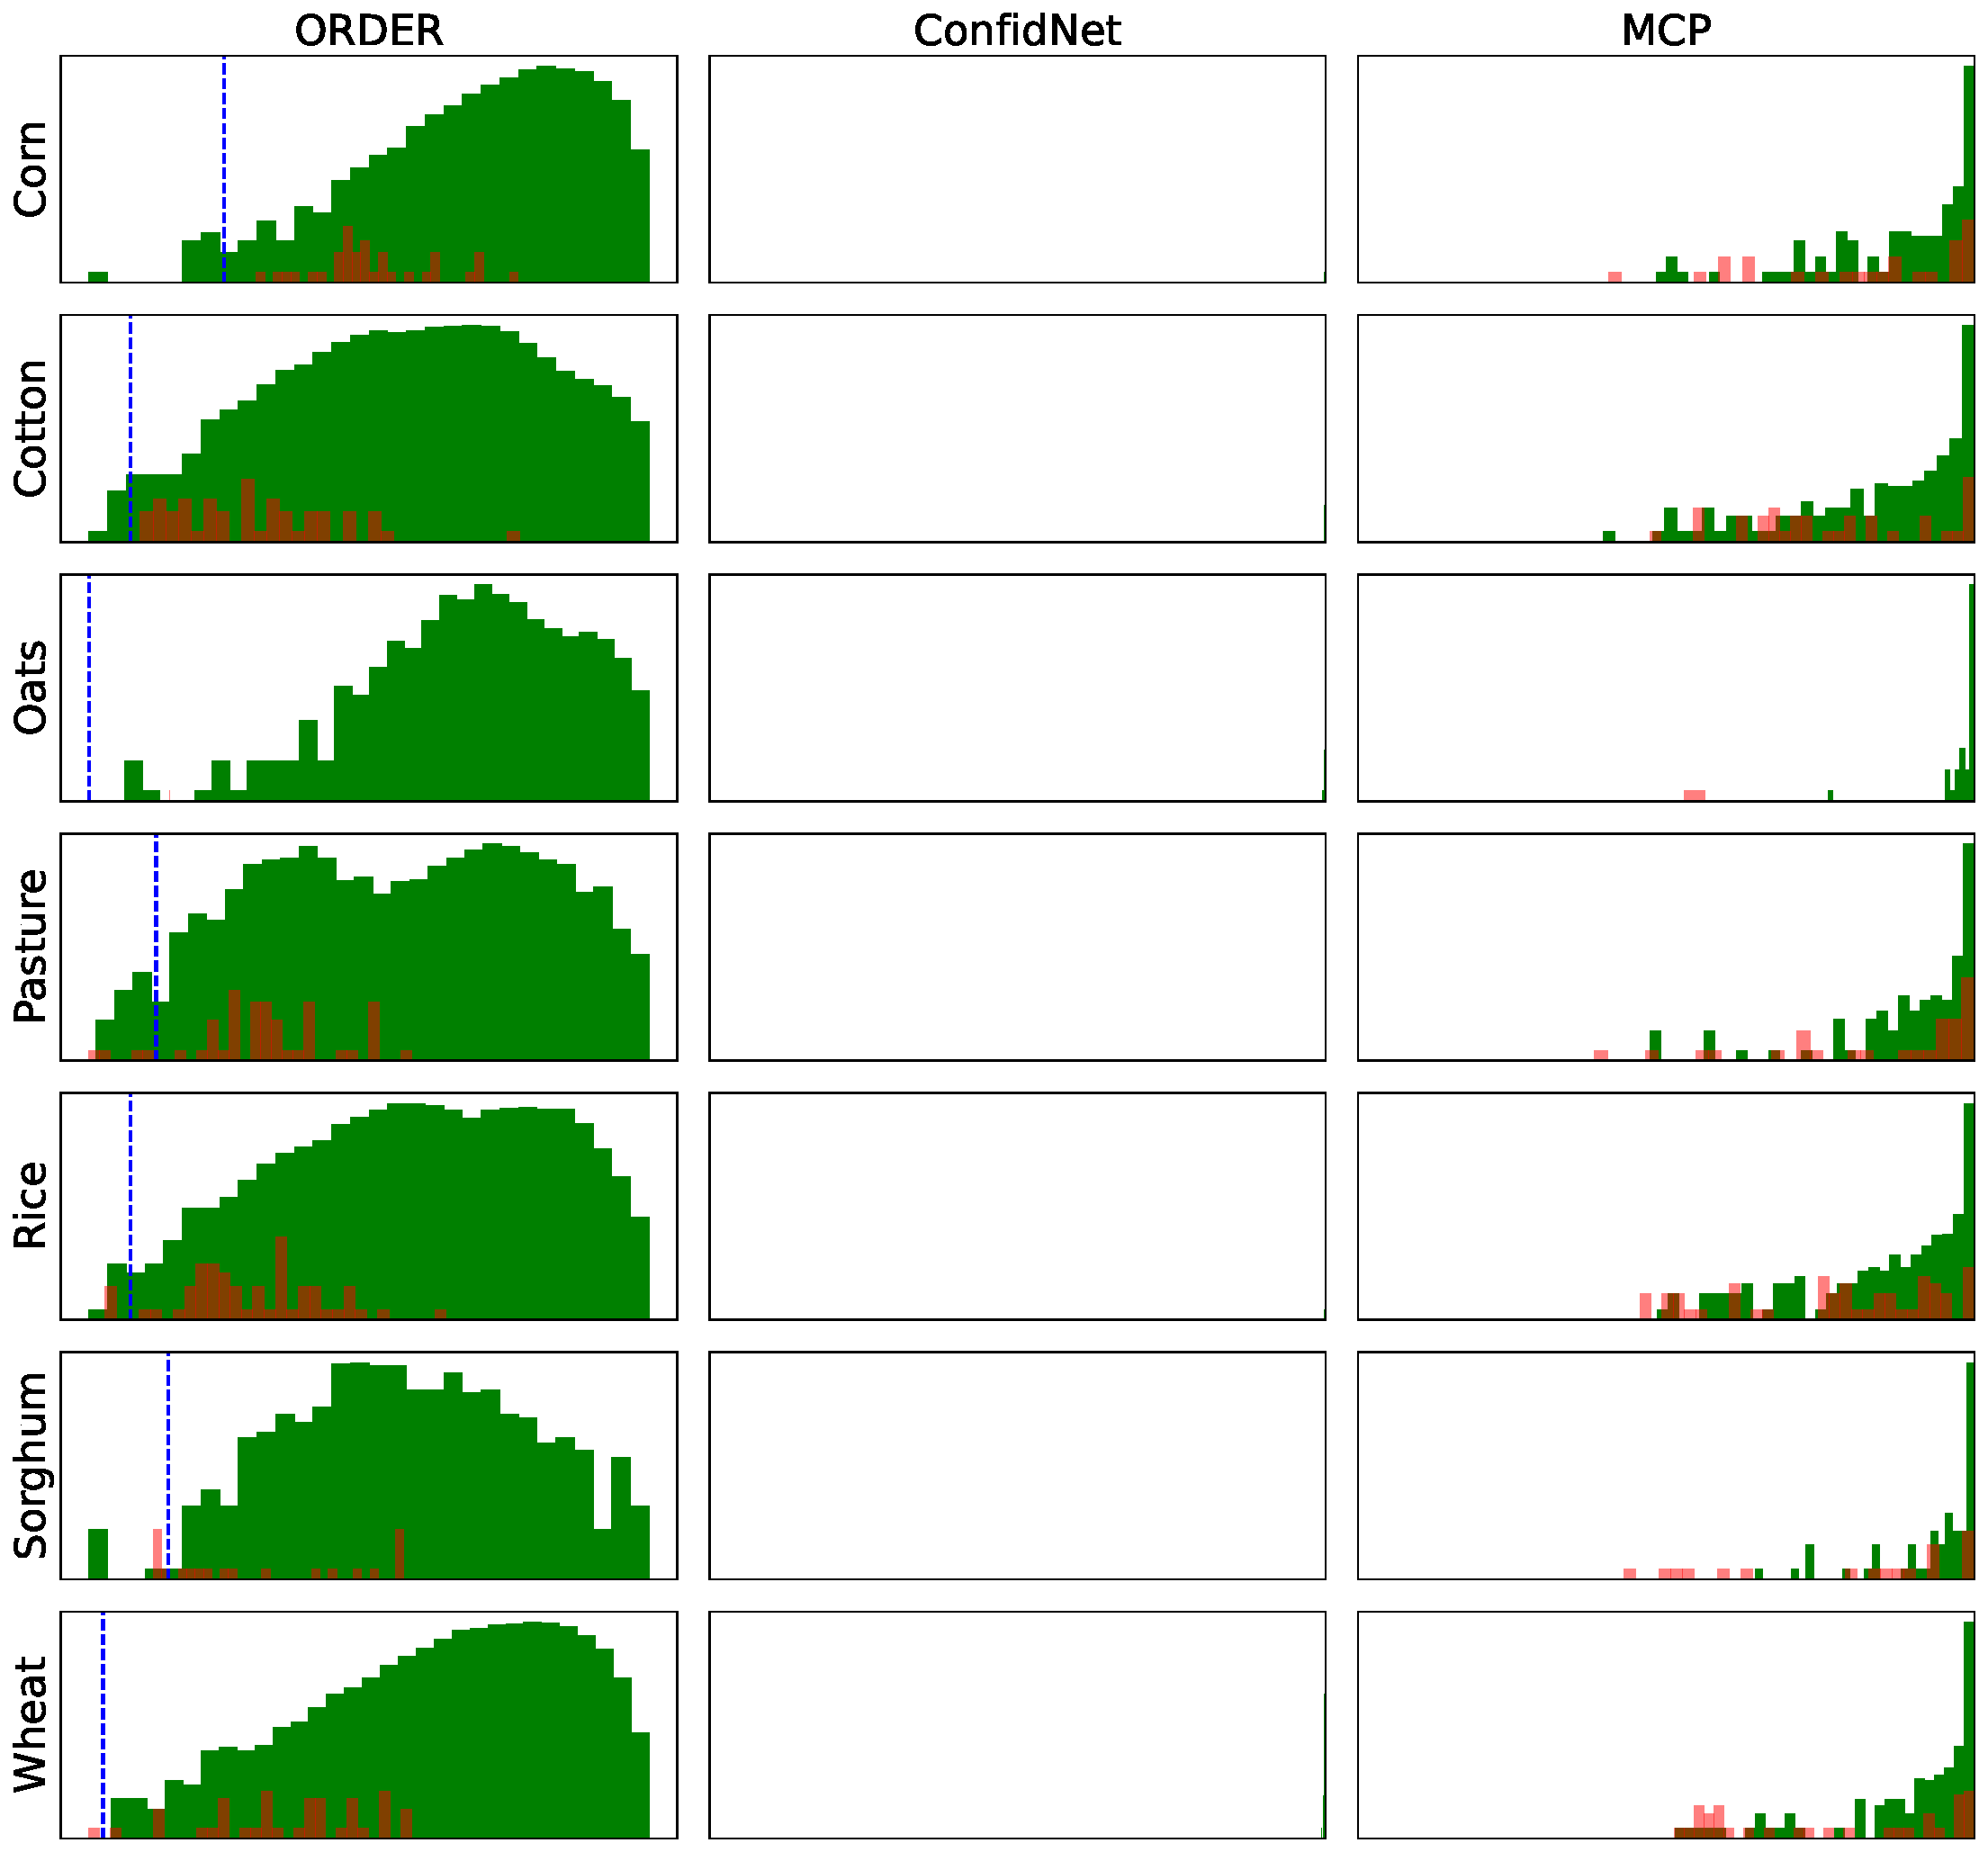
\includegraphics[width=0.6\linewidth]{figures/8_results/texas-finetuning/LSTM-70.0-FastSiam/hist_combined_test.pdf}
    \label{fig:texas_gmm}
    \fignote{Y-axis is in logarithmic scale.}
\end{figure}

Regarding the separability of correct and incorrect predictions (see \autoref{fig:texas_gmm}), the histograms from ConfidNet and MCP are difficult to visualize due to the high clustering very close to the value 1. \ac{ORDER} , however, continues to show unsaturated scores, although it is difficult to determine its efficiency due to the very low number of incorrect predictions.

\subsection{California Dataset}

\begin{figure}[ht!]
    \centering
    % Início da primeira subfigura (Matriz)
    \begin{subfigure}[b]{0.48\textwidth}
        \centering
        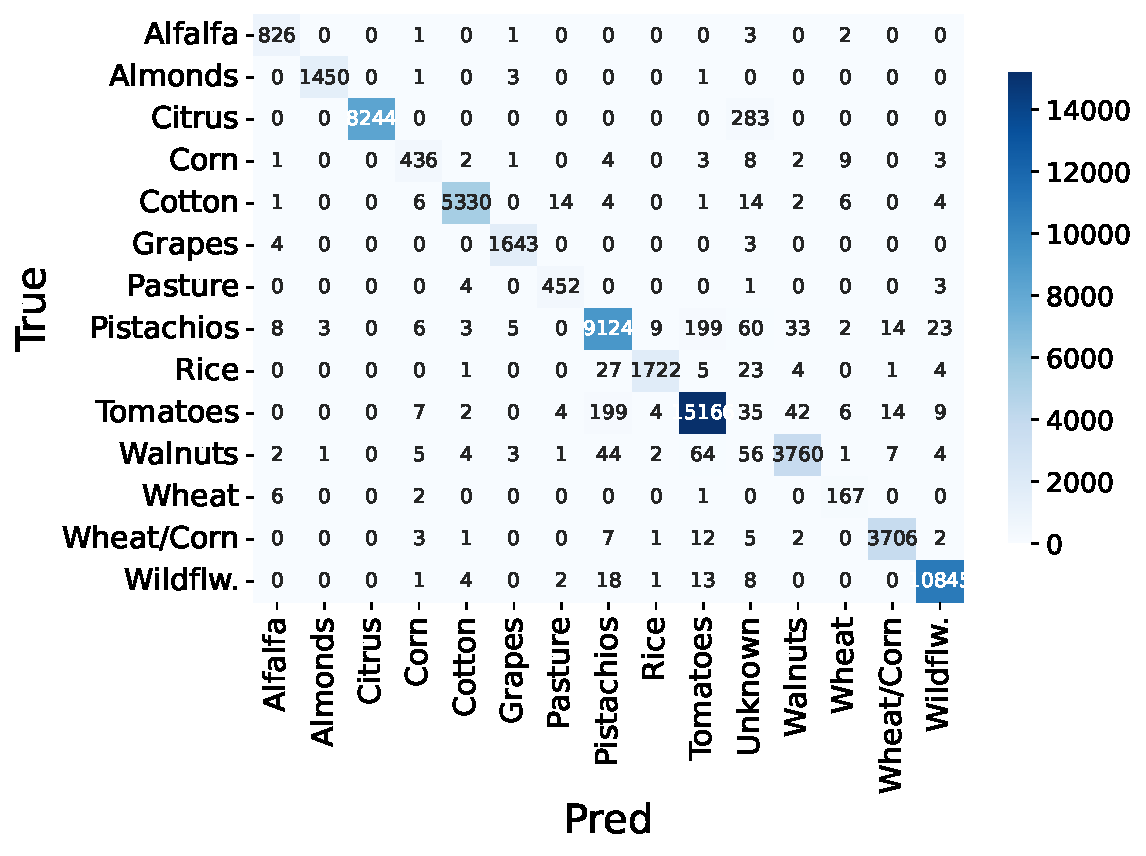
\includegraphics[width=\linewidth]{figures/8_results/california-finetuning/MAMBA-70.0-reconstruct/class_test_gemmos_matrix.pdf}
        %\caption{Matriz de Confusão}
        \label{fig:california_cm}
    \end{subfigure}
    \hfill % Adiciona espaço elástico entre as figuras
    % Início da segunda subfigura (Relatório)
    \begin{subfigure}[b]{0.48\textwidth}
        \centering
        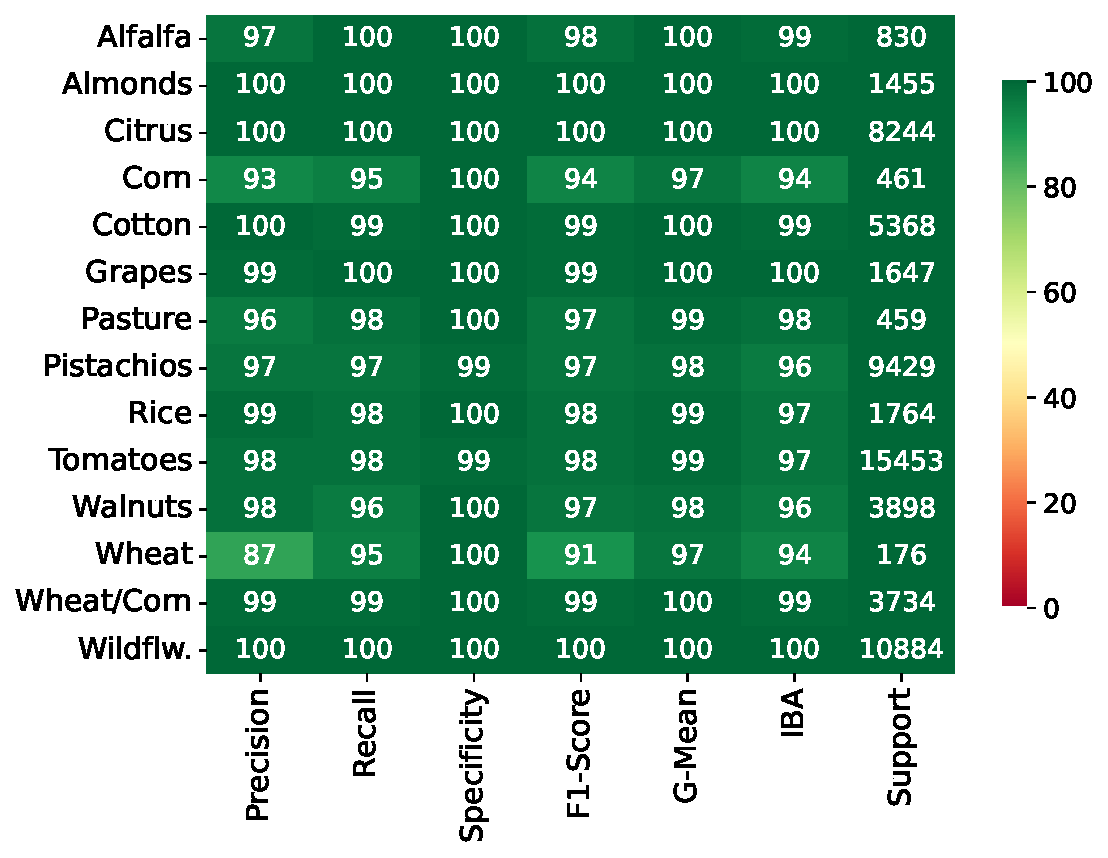
\includegraphics[width=\linewidth]{figures/8_results/california-finetuning/MAMBA-70.0-reconstruct/class_test_gemmos_report.pdf}
        %\caption{Relatório de Classificação}
        \label{fig:california_cr}
    \end{subfigure}
    
    % Legenda geral para ambas as figuras
    \caption{Best experiment in California Dataset with 70\% in training data (Mamba with MM pretraining)..}
    \label{fig:california_experiments}
\end{figure}

Doing the same with the California dataset (see \autoref{fig:california_experiments}), the best experiment on this dataset was using the Mamba model with MM pretraining, demonstrating a robust performance across most agricultural classes. The confusion matrix exhibits a well-defined main diagonal, with near-perfect classification for categories such as Almonds, Citrus, and Wildflow. There is a  consistently high and F1-Score values.

However, the analysis of misclassifications reveals specific spectral-temporal overlaps, most notably between Pistachios and Tomatoes, which accounted for the largest volume of mutual confusion. Additionally, the Wheat class presented the lowest precision (87\%), frequently being mistaken for Alfalfa or Rice, likely due to similarities in phenological cycles or its relatively lower sample support compared to dominant classes.

\begin{figure}[ht!]
    \centering
    \caption{Best experiment in California Dataset with 70\% in training data (Mamba with MM pretraining) separability between right and wrong predictions with ORDER.}
    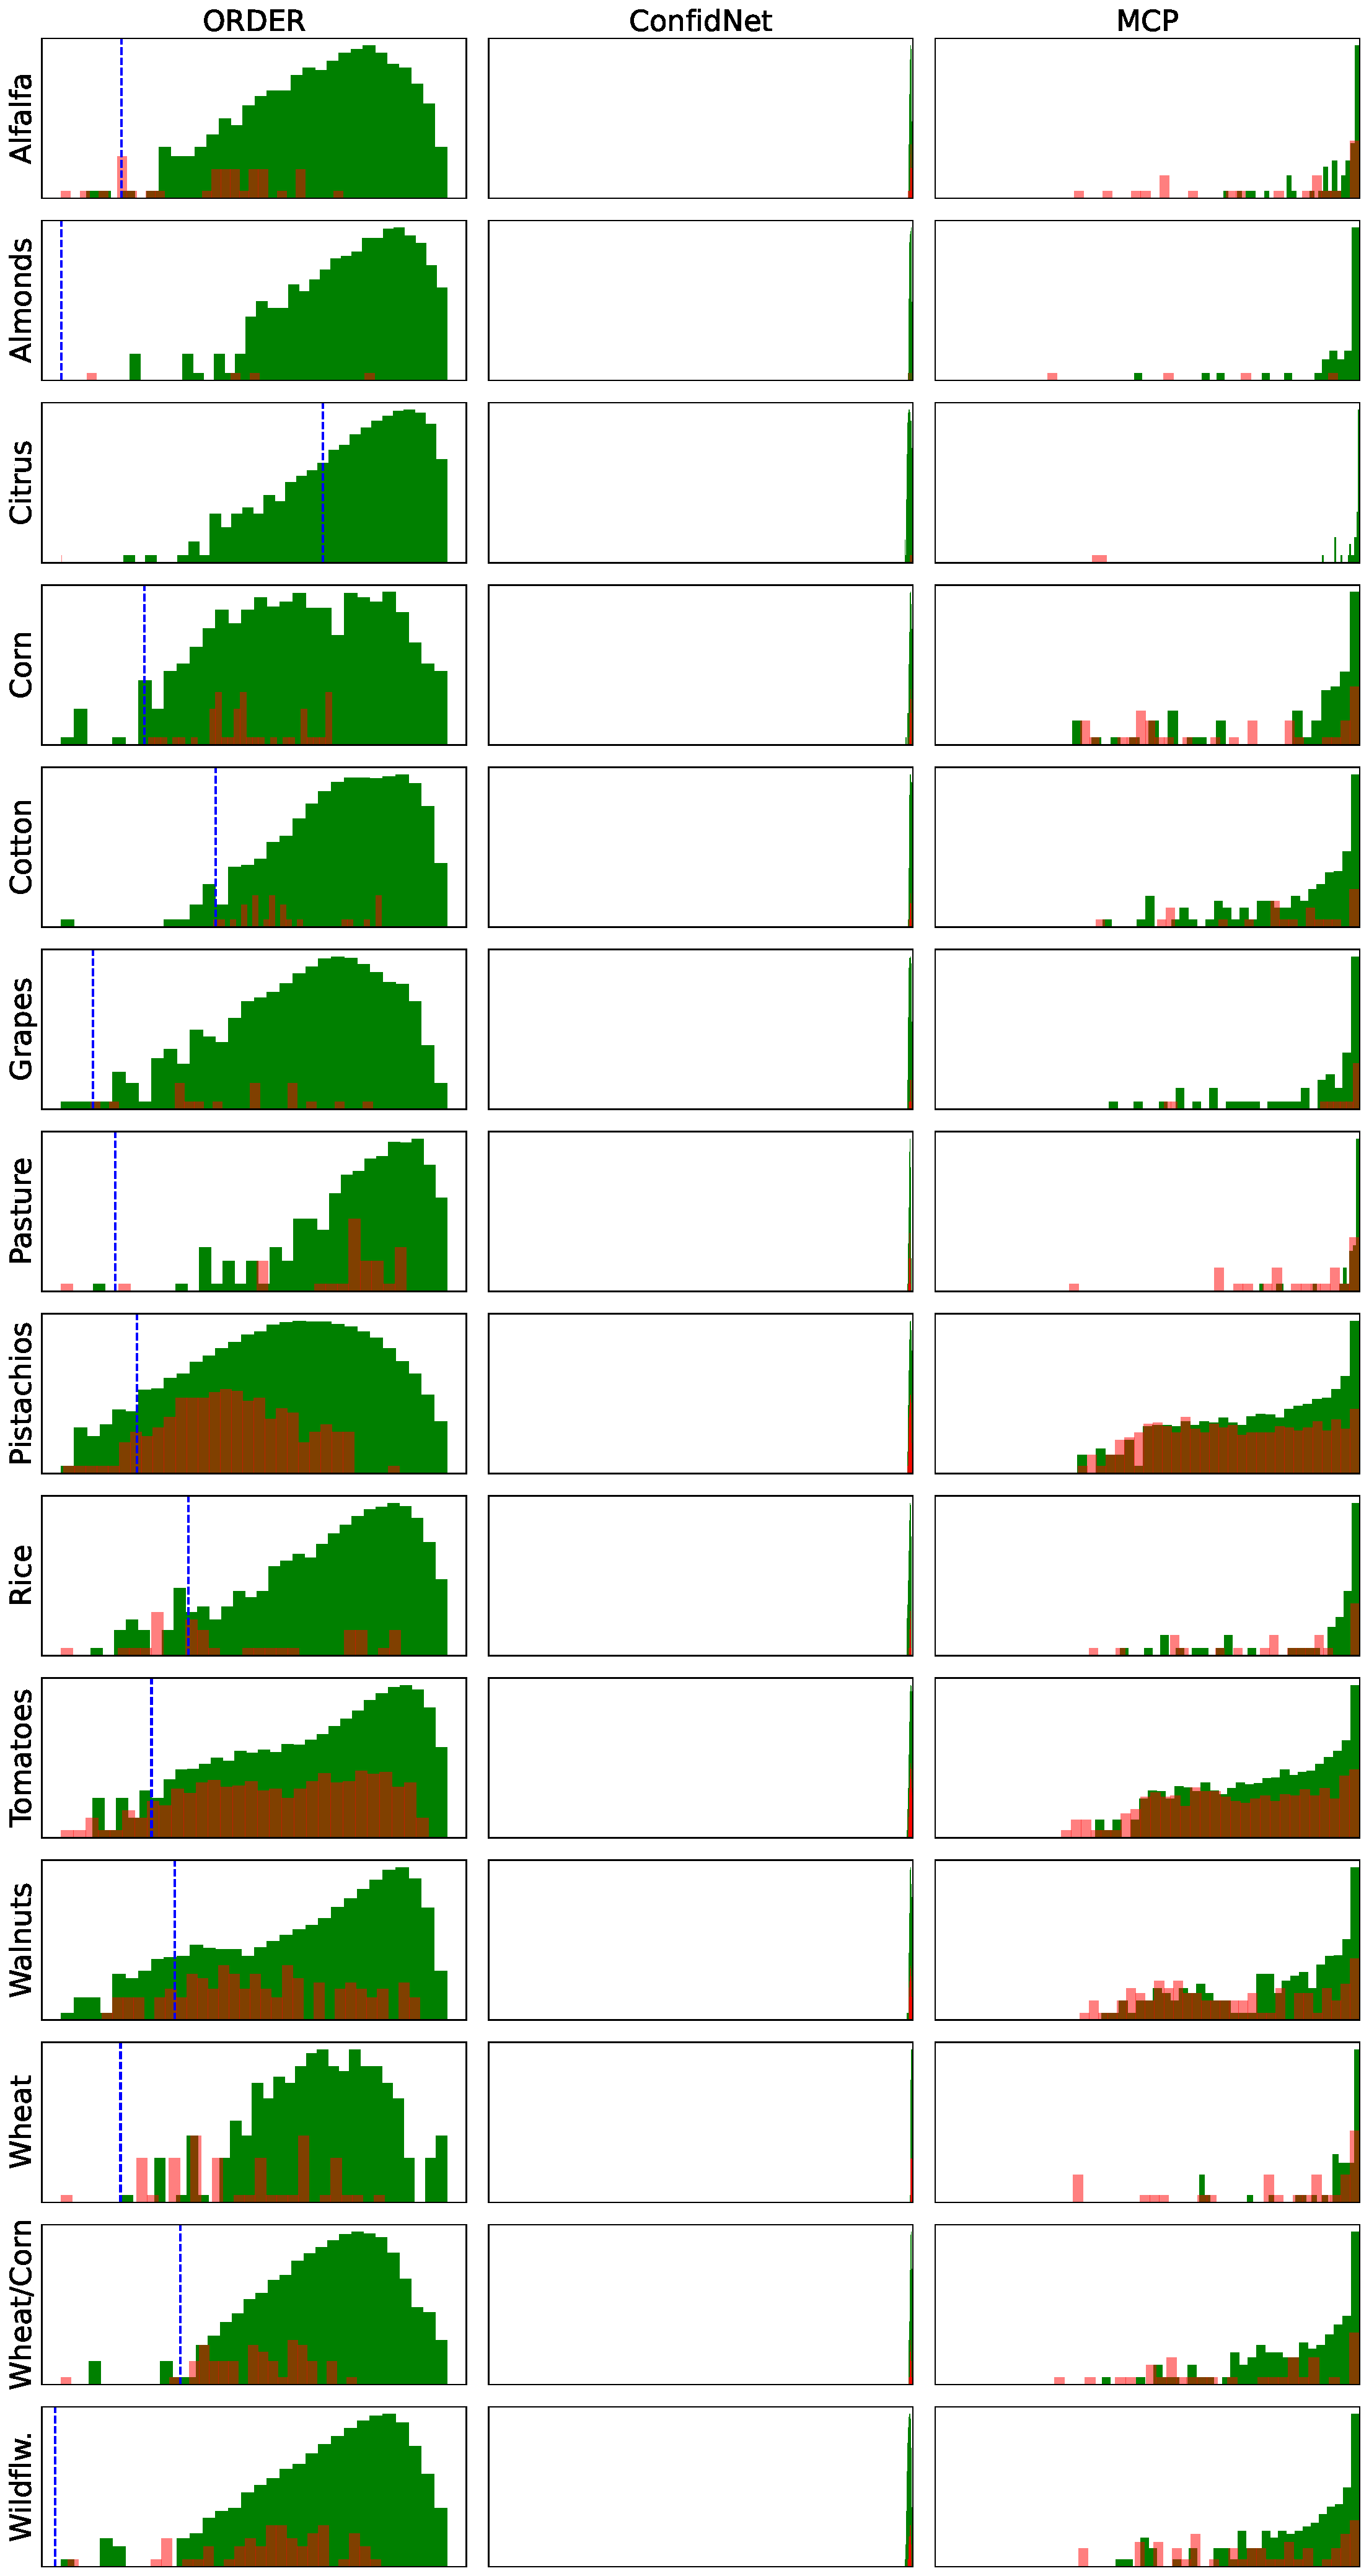
\includegraphics[width=0.6\linewidth]{figures/8_results/california-finetuning/MAMBA-70.0-reconstruct/hist_combined_test.pdf}
    \label{fig:california_gmm}
    \fignote{Y-axis is in logarithmic scale.}
\end{figure}

Again, it is very difficult to determine the effectiveness of ORDER (see \autoref{fig:california_gmm}) given a model with such high evaluation metrics. However, at least the scores are not all saturated close to 1, as is the case with ConfidNet and MCP. Thus, it seems more likely that the strategy would work if there were more challenging samples than the baselines.